

\documentclass[twocolumn,titlepage]{article}

\usepackage[a4paper,left=2cm,right=2cm,top=2.6cm,bottom=2cm]{geometry}
\usepackage[utf8]{inputenc}
\usepackage{mathrsfs}
% \usepackage{upgreek}
\usepackage{siunitx}
\usepackage{amsmath}
\usepackage{mdframed}
\usepackage{fontawesome}
\usepackage{amssymb}
\usepackage[spanish, mexico]{babel}
\usepackage{beton}
\usepackage{mathtools}
\usepackage{hyperref}
\hypersetup{
    colorlinks,
    citecolor=black,
    filecolor=black,
    linkcolor=black,
    urlcolor=black
}

\usepackage{bm}
\usepackage{cancel}

% \usepackage{unicode-math} %Terrible things
% \usepackage{fontspec}  %Cambiar compiler a LuaLatex
% \setmainfont{Comic Sans MS}% Terrible indeed
% \setmathfont{Comic Sans MS}
\usepackage{tabularx}
\usepackage{siunitx}
\usepackage{natbib}
 \bibliographystyle{plainnat} 
 
\sisetup{
detect-family,
detect-display-math = true, 
output-decimal-marker = {,} %Esto decide si el separador decimal es coma o punto
}
\usepackage[pages=some]{background}
\backgroundsetup{
scale=1.4,
color=black,
opacity=0.6,
angle=0,
position={7.93,-10.34},
contents={%
  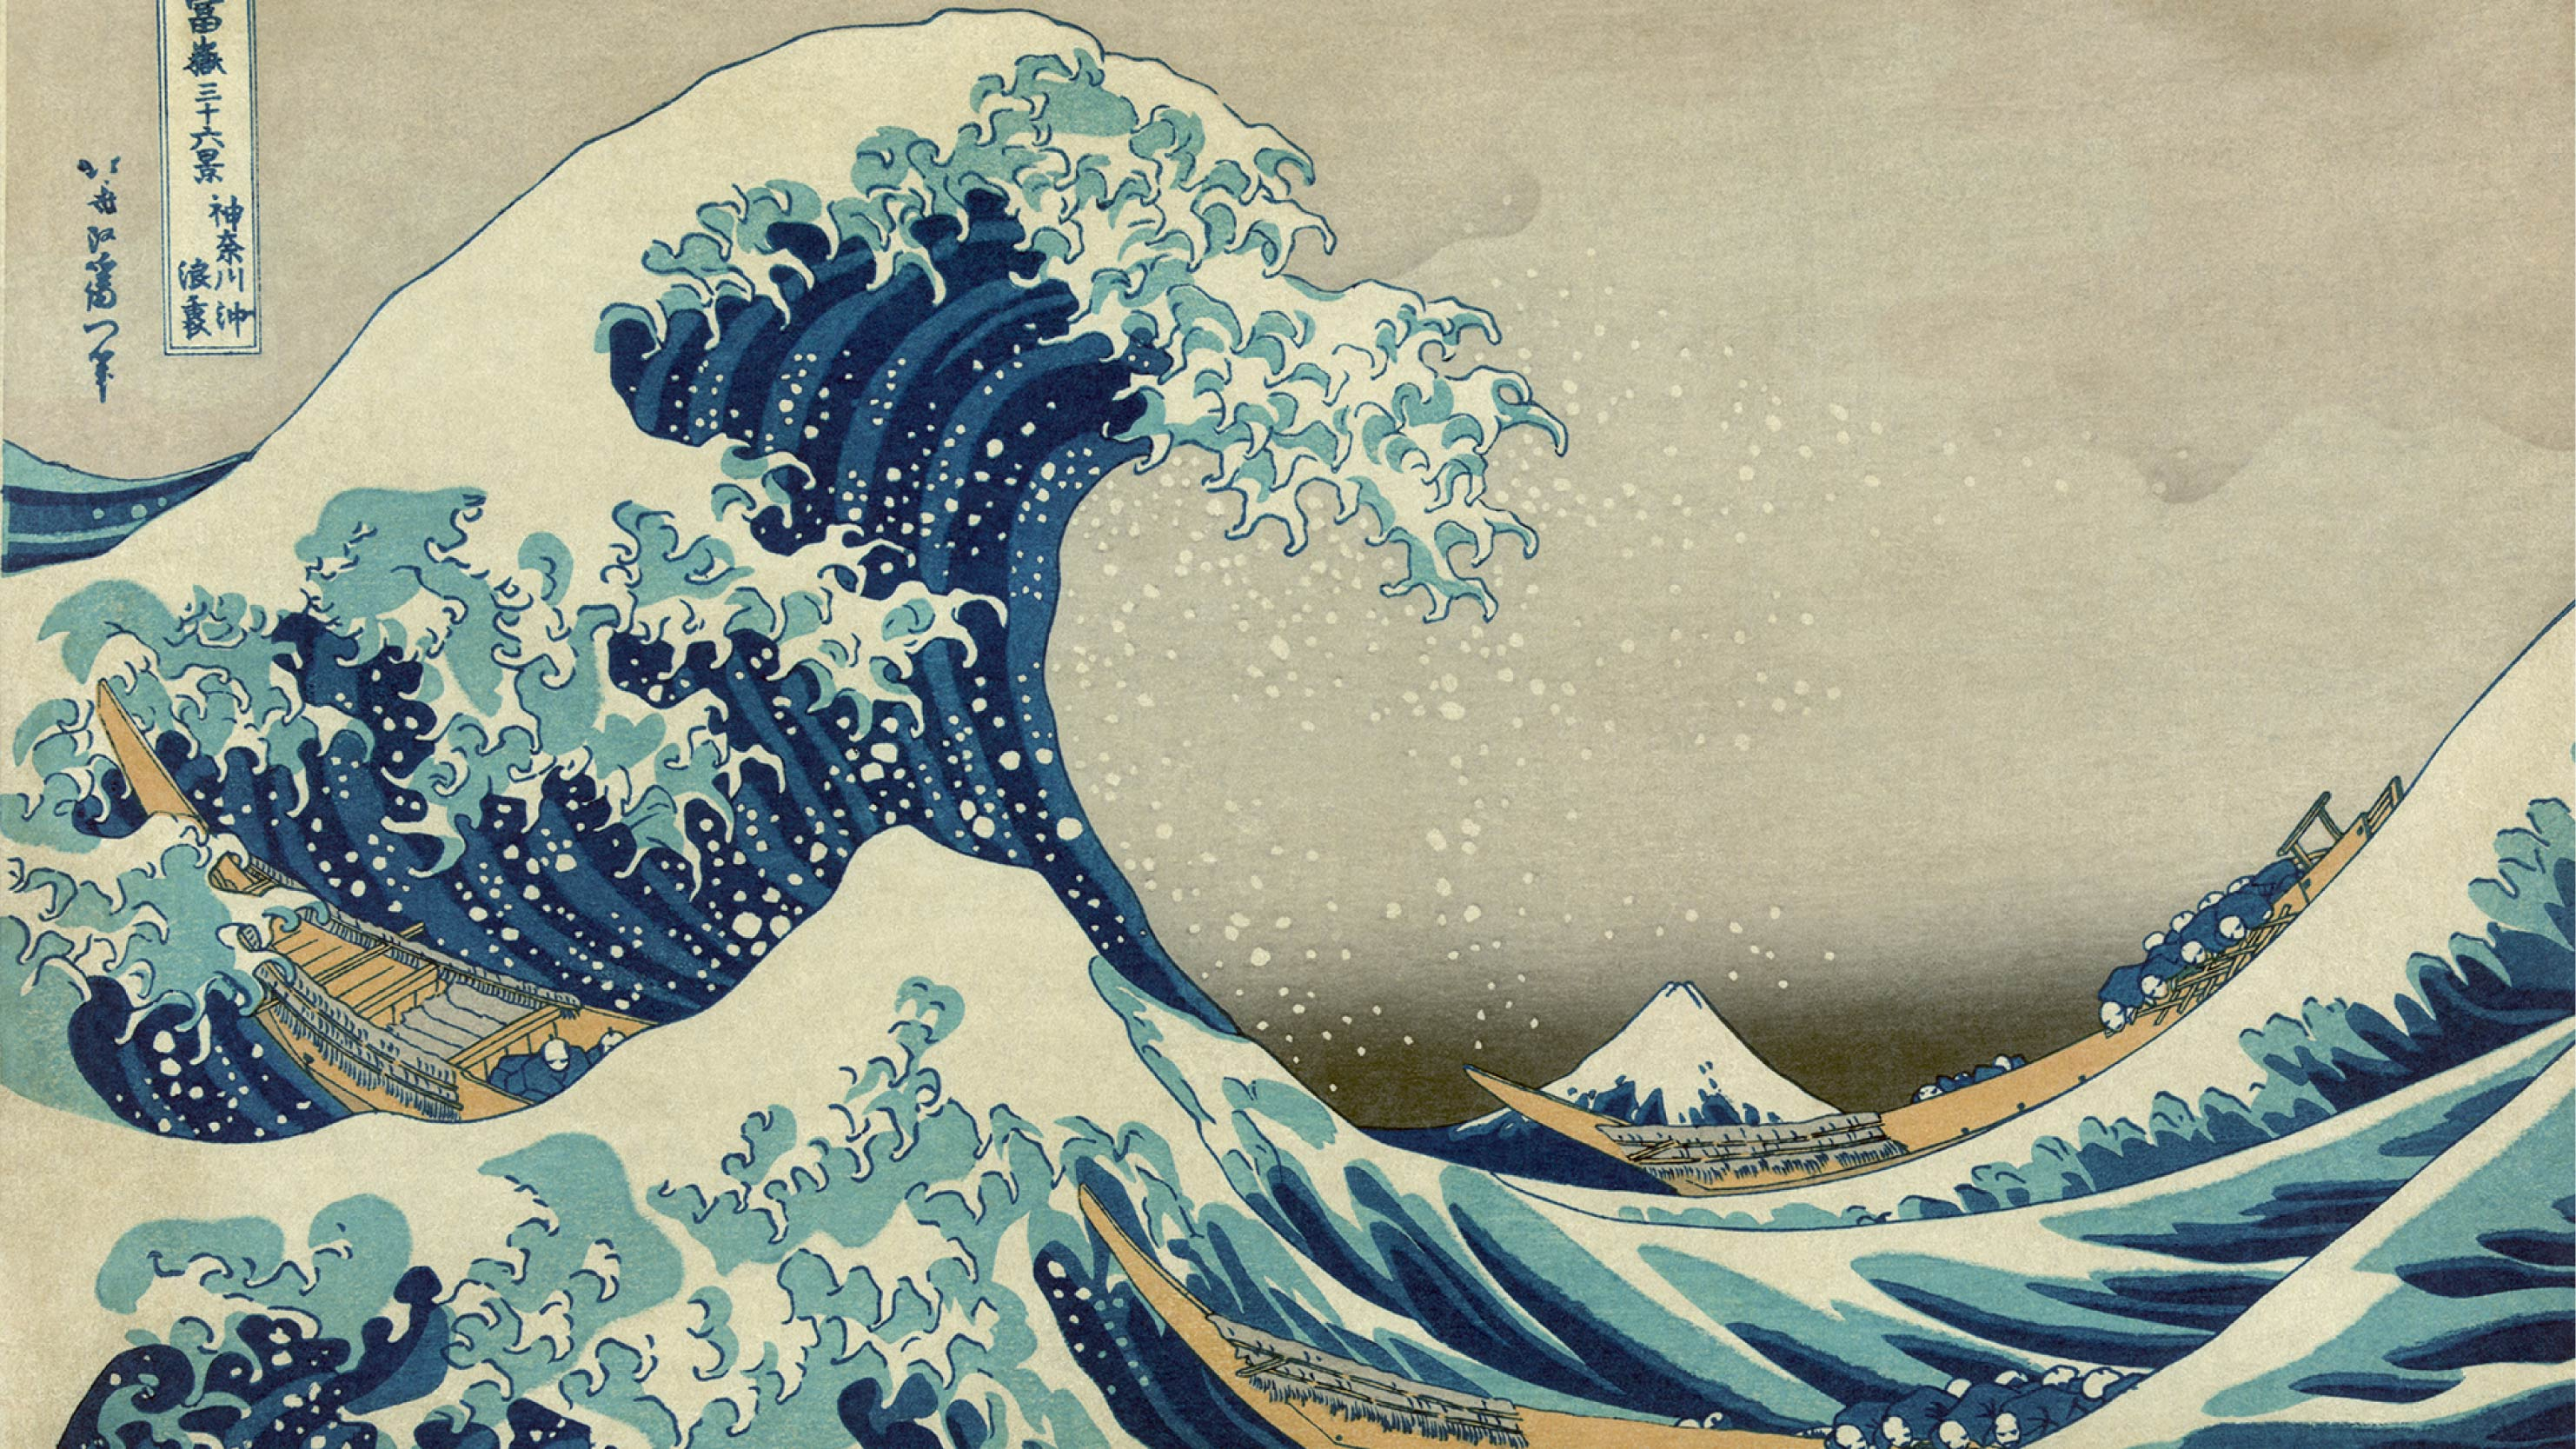
\includegraphics[width=\paperwidth]{waveoffkana.jpg}
  }%
}
\title{Resúmen Transferencia Calor}
%\renewcommand\spanishtablename{Tabla}
\newcommand\numberthis{\addtocounter{equation}{1}\tag{\theequation}}

\usepackage[mathscr]{eucal}

\newcommand{\Matlab}{\mbox{\fontfamily{cmr}\selectfont \scshape{Matlab}}}

\newcommand{\ttens}[1]{\underline{\underline{#1}}}
\newcommand{\ttensb}[1]{\underline{\underline{\mathbf{#1}}}}
\newcommand{\boltzmann}{k_{\textrm{\RM{B}}}}
\newcommand{\derpq}{\rotatebox[origin=c]{180}{?}}
\newcommand{\smol}[1]{{\mbox{\tiny $#1$}}}
\newcommand{\gradient}{\textrm{grad }}
\newcommand{\diverg}{\textrm{div }}
\newcommand{\rotor}{\textrm{rot }}

\newcommand{\RM}[1]{\mbox{\fontfamily{cmr}\selectfont\scriptsize #1}}
\newcommand{\overtilde}[1]{\widetilde{#1}}
\newcommand{\mhyph}{\mbox{ - }}
\newcommand{\Dscr}{\mathscr{D}}
\newcommand{\Uscr}{\mathscr{U}}
\newcommand{\Lscr}{\mathscr{L}}
\newcommand{\moldens}{\bar{n}}
\newcommand{\crit}{{\textrm{crit}}}
\newcommand{\pe}{p_{\mbox{\scriptsize\fontfamily{cmr}\selectfont e}}}
\newcommand{\entrada}{{\mbox{\scriptsize\fontfamily{cmr}\selectfont entrada}}}
\newcommand{\salida}{{\mbox{\scriptsize\fontfamily{cmr}\selectfont salida}}}
\newcommand{\ANPA}{{\mbox{\fontfamily{cmr}\selectfont ANPA}}}
\newcommand{\breathingspace}{\vspace{.1cm}}
\newcommand{\hhline}{\hline\vspace{-.4cm}\\\hline}
\newcommand{\promedio}{\textrm{prom.}}
% \newcommand{\salida}{\textrm{salida}}
% \newcommand{\entrada}{\textrm{entrada}}
\newcommand{\efic}{\mathcal{E}}
% \newcommand{\crit}{\textrm{\textbf{crit}}}
\newcommand{\Tfilm}{T_{\textrm{film}}}
\newcommand{\grados}{^{\circ}}
\newcommand{\di}{\textrm{d}}
\newcommand{\Di}{\textrm{D}}
\newcommand{\ek}{\textrm{e}_K}
\newcommand{\interna}{\textrm{interna}}
\newcommand{\externa}{\textrm{externa}}
\newcommand{\et}{\textrm{e}_T}
\newcommand{\ei}{\textrm{e}}
\newcommand{\hcb}{\bar{h}_c}
\newcommand{\hrb}{\bar{h}_r}
\newcommand{\hhb}{\bar{h}}
\newcommand{\Brinkmann}{\textrm{Br}}
\newcommand{\Fo}{\textrm{Fo}}
\newcommand{\Eckert}{\textrm{Ec}}
\newcommand{\frictionfactor}{f}
\newcommand{\Colburnfactor}{j_H}
\newcommand{\Peclet}{\textrm{Pe}}
\newcommand{\Froude}{\textrm{Fr}}
\newcommand{\Mach}{\textrm{M}}
\newcommand{\Grashof}{\textrm{Gr}}
\newcommand{\Rayleigh}{\textrm{Ra}}
\newcommand{\Stanton}{\textrm{St}}
\newcommand{\rst}{\left<u_j^\prime u_k^\prime \right>}

\newcommand{\Biot}{\textrm{Bi}}
\newcommand{\Nusselt}{\textrm{Nu}}
\newcommand{\vol}{\mathscr{V}}
\newcommand{\sur}{\mathscr{S}}
\newcommand{\lin}{\mathscr{L}}

\newcommand{\celsius}{^\circ\textrm{C}}
% \newcommand{\grad}{}
\newcommand{\Reynolds}{\textrm{Re}}
\newcommand{\spartial}[2]{\frac{\partial #1}{\partial #2}}
\newcommand{\dpartial}[2]{\frac{\partial^2 #1}{\partial #2 ^2}}
\newcommand{\fforma}{\mathscr{F}}
\newcommand{\Prandtl}{\textrm{Pr}}
\newcommand{\Weber}{\textrm{We}}
\newcommand{\Bond}{\textrm{Bo}}
\newcommand{\Eotvos}{\textrm{Eö}}
\newcommand{\Capillary}{\textrm{Ca}}
\begin{document}


\pagenumbering{roman}
\begin{titlepage} 

% Original titlepage author:
% Peter Wilson (herries.press@earthlink.net) with modifications by:
% Vel (vel@latextemplates.com)
%
% License:
% CC BY-NC-SA 3.0 (http://creativecommons.org/licenses/by-nc-sa/3.0/)


    \fontfamily{fourierenc}\selectfont %Elijo una fuente
    \BgThispage
    
	\centering % Centre everything on the title page
	
	%------------------------------------------------
	%	Top rules
	%------------------------------------------------
	
	\rule{\textwidth}{1pt} % Thick horizontal rule
	
	\vspace{2pt}\vspace{-\baselineskip} % Whitespace between rules
	
	\rule{\textwidth}{0.4pt} % Thin horizontal rule
	
	\vspace{0.1\textheight} % Whitespace between the top rules and title
	
	%------------------------------------------------
% 		Title
	%------------------------------------------------
	
	\textcolor{black}{ % Red font color
		{\Huge Termofluidos}\\[1.5\baselineskip] % Title line 1
		 % Title line 2
		{\Large para las masas} % Title line 3
	}
	
	\vspace{0.025\textheight} % Whitespace between the title and short horizontal rule
	
	\rule{0.3\textwidth}{0.4pt} % Short horizontal rule under the title
	
	\vspace{0.1\textheight} % Whitespace between the thin horizontal rule and the author name
	
	%------------------------------------------------
	%	Author
	%------------------------------------------------
	
% 	{\Large \textsc{Física IV -- 93.44}} % Author name
	\vspace{3cm}
    


	\vfill % Whitespace between the author name and publisher
	
    
	%------------------------------------------------
	%	Publisher
	%------------------------------------------------
	
	{\Large{\fbox{$\mathscr{WL}$}}}\\[-3\baselineskip] % Publisher logo

	
	\vspace{0.1\textheight} % Whitespace under the publisher text
	
	%------------------------------------------------
	%	Bottom rules
	%------------------------------------------------
	
	\rule{\textwidth}{0.4pt} % Thin horizontal rule
	
	\vspace{2pt}\vspace{-\baselineskip} % Whitespace between rules
	
	\rule{\textwidth}{1pt} % Thick horizontal rule
	
\end{titlepage}
\onecolumn

\begin{table}[htb!]
\vspace{-1cm}
\centering
\begin{tabularx}{12cm}{ *{2}{c}
>{\scriptsize\arraybackslash}X }
\multicolumn{3}{l}{Grupos adimensionales \citep{kreith2011principles}}\\\hline
Grupo               & Definición & \normalsize Interpretación \\\hline
Número de Reynolds ($\Reynolds$)  &   $\frac{U\rho L}{\mu}=\frac{U L}{\nu}$         &  Razón de inercia a fuerzas viscosas \breathingspace             \\
Coeficiente de drag ($C_D$)& $\frac{F_D}{\rho U_\infty A/2}$            &  Cuantifica el \textit{drag} o la resistencia de un objeto sumergido en un fluido.             \\
Número de Fourier ($\Fo$)  &    $\frac{\alpha t}{L^2}=\frac{k t}{\rho c_p L^2} $        & Razón de conducción de calor a
la acumulación de energía interna en un solido. \\
 Número de Froude    ($\Froude$)&  $\frac{U_\infty}{\sqrt{g L}}$          &   Relaciona el flujo de inercia a un campo externo (inercia de un barco perdido a su estela)            \\
Número de Nusselt  ($\Nusselt$) &   $\frac{\hcb L}{k_f}$         & Razón de transferencia de calor convección a conducción sobre una capa de fluido de longitud $L$.              \\
Número de Biot  ($\Biot$)    &     $\frac{\hhb \ell}{k_s} $      & Razón de la resistencia térmica interna de un cuerpo solido a la resistencia de su superficie.           \\
Número de Bond (Eötvös) ($\Bond$ o $\Eotvos$)    &     $\frac{\rho g \ell^2}{\Upsilon} $      & Relación de fuerzas por gravedad a las capilares.           \\
Número de Brinkmann ($\Brinkmann$) & $\frac{\mu U^2}{k_f(T_{\textrm{wall}}-T_0)}$ &Razón de calor producido por disipación viscosa a el calor transportado por conducción molecular. \\
Número capilar ($\textrm{Ca}$)& $\frac{\mu U}{\Upsilon}$            &  Razón de fuerzas viscosas con las capilares.              \\
Coeficiente de fricción ($c_f$)& $\frac{\tau_s}{\rho U_\infty/2}$            &  Razón del corte de superficie a la energía cinética del flujo.              \\
Número de Eckert  ($\Eckert$)  &    $\frac{U_\infty^2}{c_p\left(T_s-T_\infty\right)}$        &Energía cinética de un flujo relativo a la diferencia de entalpía de la capa limite. Usado para caracterizar la disipación de calor.                \\
Factor de fricción ($\frictionfactor$) & $ \frac{\Delta p}{(L/D)\left(\rho U^2_m/2\right)}$          &Caracteriza la caída de presión para flujos dentro de conductos.                \\
Número de Grashof ($\Grashof$) &  $\frac{g\beta \left(T_s -T_\infty \right) L^3}{\nu^2}$          &Razón de fuerzas de flotación a fuerzas viscosas.                \\
% Factor j de Colburn ($\Colburnfactor$)&   $\Stanton\Prandtl^{\frac{2}{3}}$         &    Coeficiente de transferencia de calor.            \\
Número de Mach   ($\Mach$)   &    $\frac{U}{U_{\textrm{sonido}}}$        & Razón de velocidad de un flujo a la velocidad de sonido local.              \\
% Número de Peclet ($\Peclet$)   &    $\Reynolds\Prandtl$        & Razón de advección a difusión de un fluido.                \\
Número de Prandtl  ($\Prandtl$) &     $\frac{\nu}{\alpha}=\frac{c_p \mu}{k}$       &Razón de difusión viscosa a difusión térmica.               \\
Número de Rayleigh ($\Rayleigh$) &  $\Grashof\Prandtl = \frac{\Delta \!T g\beta L^3}{\nu \alpha}$          & Caracteriza el flujo impulsado por el fenómeno de flotación o empuje. Asociado a la convección natural.             \\
Número de Stanton ($\Stanton$)  &   $\frac{\hcb }{\rho U_\infty c_p}=\frac{\Nusselt_L}{\Reynolds_L \Prandtl}$         &Razón de transferencia de calor a capacidad térmica de un fluido. Asociado a convección forzada.\\
Número de Weber ($\Weber$)  &   $\frac{\rho U^2 L}{\Upsilon}$         &Razón de fuerzas de inercia en un flujo a la capilar.\\
\hhline
\end{tabularx}
\end{table} 

\tableofcontents

\section*{Sobre esta obra}
Documento escrito en \textrm{\LaTeX} usando \href{https://www.overleaf.com}{Overleaf}. Caratula: \emph{ La Gran Ola de Kanagawa }- Katsushika Hokusai. \par

Sepa diferenciar $\nu$ (nu) de $v$ (uve).\par
 \vspace{.1cm}
\fbox{Versión: \today}
 \vspace{1cm}
 \begingroup

\fontfamily{pbk}\selectfont
\noindent
 Licencia: CC-BY-NC-SA 4.0
 \endgroup
 \begingroup
    $$\textrm{N--S 2-D}_x:\quad \spartial{u}{t}+u\spartial{u}{x}+v\spartial{u}{y}=b_x-\frac{1}{\rho}\spartial{p}{x}+\frac{\mu}{\rho}\left(\dpartial{u}{x}+\dpartial{u}{y}\right) + \frac{\mu}{3}\spartial{ }{x}\left( \spartial{u}{x}+\spartial{v}{y}\right)$$
 \endgroup%Titulo y primera parte
%\pagestyle{plain}
\twocolumn
\setcounter{page}{1}
\pagenumbering{arabic}

%%%%%%%%%%%%%%%%%%%%%%%%%%%%%%%%%%%%%%%%%%%%%%%%%%%%%%%%%
\part{Mecánica de Fluidos}
\section{Introducción a la mecánica de fluidos}
\subsection{Repaso de tensores cartesianos}
\[
a_i =\vec{a}= \begin{Bmatrix}
a_1 \\
a_2 \\
a_3
\end{Bmatrix}% \left\{ a_1,\; a_2, \; a_3\right\}
\]
\[
\gradient a_i=\nabla a_i = 
\begin{Bmatrix}
\vspace{.1cm}\spartial{a_1}{x_1} \\
\vspace{.1cm}\spartial{a_2}{x_2} \\
\spartial{a_3}{x_3}
\end{Bmatrix}%\left\{ \spartial{a_1}{x_1},\;\spartial{a_2}{x_2},\;\spartial{a_3}{x_3} \right\}
\]

\[
\diverg a_i = \nabla \cdot a_i=\nabla_k a_k=\partial_k a_k =\spartial{a_1}{x_1}+\spartial{a_2}{x_2}+\spartial{a_3}{x_3}
\]

\[
\rotor a_i = \nabla \times a_i  = -\epsilon_{ijk} \spartial{a_i}{x_j}= \epsilon_{ijk} \spartial{a_j}{x_i}
\]
El operador laplace:
\[
\nabla^2 a_i= \begin{Bmatrix}
\nabla^2 a_1 \\
\nabla^2 a_2 \\
\nabla^2 a_3
\end{Bmatrix} 
\]
donde
\[
\nabla^2 a = \dpartial{a}{x_1}+\dpartial{a}{x_2}+\dpartial{a}{x_3}=\frac{\partial^2 a}{\partial x_i \partial x_i} 
\]

La delta de Kronecker (matriz identidad):
\[
\delta_{ij}=\mathbf{I}=\begin{bmatrix}
1 & 0& 0\\
0 & 1 & 0\\
0 & 0 &1
\end{bmatrix}
\]
\subsection{Conceptos físicos básicos}
\subsubsection*{La materia}

Estados de agregación de la materia
\begin{itemize}
    \item Condensado de Bose-Einstein
    \item Sólido
    \item Liquido
    \item Gas
    \item Plasma 
\end{itemize}



Las fuerzas intermoleculares para moléculas de gas no-polares \citep{bird2002transport}: 

\[
F_r(r)=\frac{24 \epsilon}{r_{\min}}\left[ 2\left( \frac{r_{\min}}{r}\right)^{13} - \left( \frac{r_{\min}}{r} \right)^7 \right]
\]
dado por el \textit{potencial} $U_r$ \textit{de} \textit{Lennard-Jones}:
\[
U_r(r) = 4\epsilon \left[ \left(\frac{r_{\min}}{r}\right)^{12} - \left( \frac{r_{\min}}{r}\right)^6 \right] 
\]

En contraste a los sólidos, cuando un fluido recibe tensiones de corte, va tender a fluir. Por ende se puede inferir que un fluido en reposo \textbf{no} tiene tensiones de corte. 

Como toda materia consiste de moléculas, toda propiedad macroscópica puede ser descrita por propiedades moleculares pero, debido a la dificultades que surgen de un tratamiento molecular, se opta por la mecánica del continuo para describir propiedades del fluido\citep{durst2008fluid}. 
\subsubsection*{Modelo gas ideal}

Las leyes de los gases ideales están basadas en las leyes mecánicas para esferas que se mueven en el espacio \citep{durst2008fluid}.
\begin{itemize} 
    \item[Hip. I)] El volumen de los átomos y/o moléculas es extremadamente pequeño en comparación con la distancia entre ellos
    \item[Hip. II)] No hay fuerzas atractivas ni repulsivas ejercidas entre las moléculas excepto en el momento de choque
    \item[Hip. III)] Para la colisión entre dos moléculas, o una molécula y una pared, valen las leyes de colisiones perfectamente elásticas 
\end{itemize}

Ley para gases ideales:

\begin{equation} \label{eq:idealGasesLaw}
    \pe= \moldens \boltzmann T=\frac{N\overtilde{R}T}{V}
\end{equation}
donde $\boltzmann$ es la constante de Boltzmann y vale $\SI{1.380649e-23}{\meter \squared \kilogram \per \second \squared \per \kelvin}$. $\moldens$ es la cantidad de moléculas de gas por unidad volumen. $N$ es la cantidad de moles. $R$ es la constante de gas ideal universal $\overtilde{R}=\SI{8,31447}{\joule \per \mole \per \kelvin}$. $\pe$ es la \textbf{presión termodinámica}

Existe también la expresión especifica de la ley para gases ideales
\[
\pe = \frac{RT}{v} = \rho R T
\]
donde $v=\frac{1}{\rho}$ es el volumen especifico y  $R$ [\si{\joule \per \kilogram \per \kelvin}] es la constante especifica del gas.

Generalmente el contenido de energía de un gas ideal está dado por
\begin{equation}
    e_{gas}=\frac{\alpha}{2}\boltzmann T
\end{equation}
donde $\alpha$ indica los grados de libertad del movimiento molecular. $\alpha=3$ para gases monoatómicos, $\alpha=5$ para gases diatómicos y $\alpha=6$ para gases triatómicos y poliatómicos.

En el estado gaseoso las moléculas tienen un movimiento aleatorio cuya velocidad promedio puede dar cero, pero la velocidad cuadrática media viene dada por
\[
\langle U^2 \rangle = \frac{3\overtilde{R}T}{M} \Rightarrow \quad U_{cm}=\sqrt{\frac{3\overtilde{R}T}{M}}
\]

\subsection{Modelo continuo}
Partimos definiendo un volumen de forma de cubo en nuestro fluido de lado $\Delta$ tal que su volumen es $\Delta^3$. La \textbf{densidad}  dentro de nuestro cubo virtual está dado por $\rho_\Delta$ 
\[
\rho_\Delta = \frac{m\cdot N_\Delta}{\Delta^3} \quad \textrm{en} \quad [\si{\kilogram \per \meter \cubed}]
\]
donde $m$ es la masa de una sola molécula, $N_\Delta$ es la cantidad de moléculas en el cubo virtual mencionado anteriormente.

Si partimos de un tamaño muy pequeño tendremos que varía mucho la densidad de moléculas en nuestro cubo. Mientras aumentamos $\Delta$ irá disminuyendo la variación hasta que sea cuasi-constante el valor de $\rho_\Delta$. 

\subsubsection*{Camino libre entre moléculas}
La materia podrá suponerse un continuo cuando $K_n\lesssim 0,1$ (Número de Knudsen)
\[
K_n = \frac{\lambda}{L}
\]
donde $\lambda$ es el camino libre medio entre colisiones y $L$ es la dimensión lineal característica.\footnote{Diámetro del tubo, ancho de caja etc.}

El camino libre medio $\lambda$ se puede calcular con la expresión
\[
\lambda = \frac{1}{\sqrt{2} \pi d^2 \moldens}
\]
donde $d$ es el diámetro molecular y $\moldens$ la densidad de partículas en un volumen. $\moldens$ es proporcional a $\frac{p}{T}$ luego $\lambda \propto \frac{T}{p}$

Para el aire tenemos $\moldens \approx \num{2,5e25}$, $d\approx \num{4e-10}$ según fuentes on-line $\Rightarrow \lambda_{\textrm{aire}} \approx \SI{5,6e-8}{\meter}=56\si{\nano \meter}$
\begin{mdframed}
A partir de aquí se comienza el tratamiento \textit{continuo} del fluido. Es decir, toda expresión consiguiente vale para volúmenes de control donde la longitud característica ceda $K_n \lesssim 0,1$!
\end{mdframed}

\subsection{Tensiones}
Las componentes de $\ttens{\sigma}$ (o $\sigma_{ij}$) representan la componente $i$ que aparece sobre una superficie orientada por el vector normal $n_j$ a esa superficie. Las fuerzas por unidad de superficie $\underline{f}$ están dadas por:
\[
\underline{f}=
\begin{Bmatrix}
f_1 \\
f_2 \\
f_3
\end{Bmatrix} =
\begin{bmatrix}
\sigma_{11} & \sigma_{12} & \sigma_{13} \\
\sigma_{21} & \sigma_{22} & \sigma_{23} \\
\sigma_{31} & \sigma_{32} & \sigma_{33} \\
\end{bmatrix} \cdot
\begin{Bmatrix}
n_1 \\
n_2 \\
n_3
\end{Bmatrix}
\]

El tensor de esfuerzos se puede separa en su parte isótropa (hidrostática) $\ttens{\sigma}^H$ y no isótropa (o desviadora) $\ttens{S}$ tal que $\ttens{\sigma}=\ttens{\sigma}^H+\ttens{S}$ con
\[
\sigma_{ij}^H=\sigma_m \cdot \begin{bmatrix}
1 & 0 & 0 \\
0 & 1 & 0 \\
0 & 0 & 1
\end{bmatrix}
\]
donde $\sigma_m = \frac{1}{3}\sigma_{kk}$ y 

\[
S_{ij}= \begin{bmatrix}
\sigma_{11}-\sigma_m & \sigma_{12} & \sigma_{13} \\
\sigma_{21} & \sigma_{22}-\sigma_m & \sigma_{23} \\
\sigma_{31} & \sigma_{32} & \sigma_{33}-\sigma_m 
\end{bmatrix}
\]

Cabe destacar que $\ttens{\sigma}^H$ contempla las componentes normales y está asociado al equilibrio del fluido mientras que $\ttens{S}$ se relaciona a los esfuerzos tangenciales y está asociado a un gradiente de velocidades. Se los suele denominar el \textbf{tensor hidrostático} y el \textbf{tensor de desviaciones}, respectivamente. 

La presión mecánica se define como $p=-\sigma_m$. Si el sistema está en equilibrio (mecánico y termodinámico) entonces $p$ resulta ser la presión termodinámica. Si $\ttens{S}=\pmb{0}$ se puede inferir que el fluido está en equilibrio hidrostático ($p=\pe$), pero no necesariamente en reposo.
 \label{sec:presionmecanica}
 

\subsection{Reología} \label{sec:reologia}
La reología es la rama de la física encargada del estudio de la deformación y flujo de la materia. Para un fluido newtoniano con solo una componente de velocidad $U_q$ se puede definir
\begin{equation}
    \tau_{pq}=-\mu \spartial{U_q}{x_p}
\end{equation}
donde $\mu$ es la \textbf{viscosidad dinámica}, $p$ indica la dirección del transporte molecular (normal a la velocidad [ver nota \ref{foot:transporteMolecular}]) y $q$ indica el componente de velocidad.

En general para fluidos
\begin{equation}
    \tau_{ij}=-\mu \left( \spartial{u_j}{x_i}+\spartial{u_i}{x_j}\right) -\lambda \delta_{ij} \spartial{u_k}{x_k}
\end{equation}
donde $\lambda$ es conocida como la \textit{segunda viscosidad}, \textit{viscosidad de expansión/dilatación} o viscosidad de volumen \citep{durst2008fluid}. Para resolver problemas de fluidos no se suele disponer del valor de $\lambda$. Para gases ideales monoatómicos $\lambda \equiv 0$ y si se trabaja con un flujo incompresible entonces se tiene que $\spartial{u_k}{x_k}=0$ y por lo tanto el término asociado es cero. La segunda viscosidad es importante para el comportamiento de gases poliatómicos ante vibraciones de altas frecuencias (absorción de ruido) y cuando se quiere describir un liquido con burbujas.

\begin{itemize}
    \item Para los gases: $\mu$ aumenta con el aumento de la temperatura
    \item Para los líquidos: $\mu$ disminuye con el aumento de la temperatura
\end{itemize}
\subsubsection*{Explicación viscosidad}
Los términos de $\tau_{ij}$ usados en mecánica de fluidos \textbf{no son} considerados como a causa de fricción \citep{durst2008fluid}! 

La viscosidad se puede describir como un intercambio de masa al nivel molecular\footnote{Dicho intercambio se suele denominar \textbf{transporte molecular.} \label{foot:transporteMolecular}} entre dos capas de un fluido que se mueven a distintas velocidades en el mismo sentido. Por consecuencia de esta diferencia de velocidades entre capas, dicho proceso conlleva también un \textbf{intercambio de cantidad de movimiento}. La capa mas rápida se \textit{desacelera} y la mas lenta se \textit{acelera} en dirección de la velocidad del flujo. De aquí surgen las ``tensiones"{} tangenciales.\footnote{Más que tensiones, $\tau_{ij}$ representa el transporte de cantidad de movimiento por unidad de área por unidad de tiempo.}


\subsubsection*{Relación constitutiva}
La relación constitutiva para fluidos de interés industrial con comportamiento \textit{independiente del tiempo} esta dada por

\[
\sigma_{ij}=\sigma_0+K\dot{\gamma}_{ij} \left| \dot{\gamma}_{ij}\right|^{n-1}
\]
donde $\sigma_0$ es la tensión de fluencia\footnote{Para fluidos del tipo plástico real y Bingham}, $K$ es denominado el índice de consistencia, $n$ es el índice reológico\footnote{$n=1$ para fluidos newtonianos y Bingham. Si $n>1$ el fluido es dilatante. Si $n<1$ el fluido es plástico.} y $\dot{\gamma}$ es la velocidad de deformación tal que $\dot{\gamma}_{ij}=\frac{1}{2}\left( \spartial{u_i}{x_j}+\spartial{u_j}{x_i}\right)$. Luego, en las secciones \ref{sec:CinematicaDeElementosdeFluido} y \ref{sec:NewtonTTR}, se definirá (y se hallará por ``casualidad", respectivamente) un tensor idéntico $e_{ij}$.

Se define la \textbf{viscosidad aparente} como $\eta$ y depende de la velocidad de deformación\footnote{Para fluidos no-newtonianos.} y del estado termodinámico ($p,T$).
\[
\eta=K\left| \dot{\gamma} \right|^{n-1}
\]
para fluidos newtonianos $K$ es constante y vale dos veces las \textbf{viscosidad dinámica}: $K=2\mu$.

\begin{figure}[htb!]
	\centering
	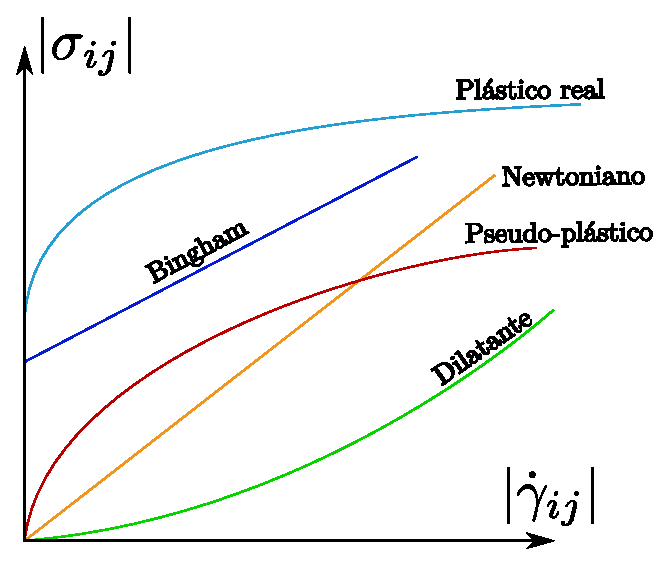
\includegraphics[width=.49\textwidth]{fig/deformacion-tensionFluidos.eps}
	\caption{Gráfico tensión-velocidad de deformación para un fluido newtoniano y varios no-newtonianos.}
\end{figure}

\derpq Alguna vez quisiste servir kétchup que tardaba en salir de la botella al principio y después de unos segundos salía a los chorros? 

Esto es un ejemplo de comportamiento \textbf{dependiente del tiempo}.\footnote{Cabe destacar que el comportamiento dependiente del tiempo es característica no-newtoniana pero no todos los fluidos no-newtonianos son dependientes del tiempo.} Para estos fluidos la viscosidad aparente depende del tiempo durante el cual el fluido es sometido a esfuerzo. La viscosidad de los fluidos \textbf{tixotrópicos} disminuye con el tiempo (kétchup) y para los \textbf{reopécticos} aumenta con el tiempo.

\subsection{Tensión superficial}
Así como hay fuerzas que actúan sobre volumen $F_\smol{V}=\rho g\cdot V$ (gravedad) y superficie $F_\smol{S}=p\cdot S$ (presión), existen fuerzas que actúan sobre \textit{longitudes}. Para el caso de los fluidos, es la \textbf{tensión superficial}. Esta fuerza la solemos despreciar en nuestro día a día, pero cuando se tienen sistemas microscópicos, esta fuerza domina.
\[
F_\smol{L} = \Upsilon L
\]%fighere
donde $\Upsilon$ (Ípsilon) es una propiedad del interfaz entre el liquido y el gas. $\Upsilon$ también depende de las propiedades termodinámicas de los fluidos. Para agua en contacto con aire a CNPT $\Upsilon=\SI{7,28e-2}{\newton \per \meter}$.

Comparamos un volumen dado por un cubo ``pequeño'' de 1mm de lado con otro ``grande'' de 1m. Para el cubo pequeño
\vspace{-.2cm}
\[V_p=1\si{\milli \meter \cubed},\, S_p=6 \si{\milli \meter \squared},\, L_p = 12 \si{\milli \meter} \]
y para el cubo grande tenemos
\vspace{-.2cm}
\begin{gather*}
    V_g=\SI{1e9}{\milli \meter \cubed},\, S_g=\SI{6e6}{\milli \meter \squared},\\ L_g =\SI{12e3}{\milli \meter}
\end{gather*}
con esto resulta aparente que la relación de fuerzas $\frac{F_\smol{L}}{F_\smol{V}}$ disminuye fuertemente con el aumento del tamaño característico del problema. Para el rango de número de Bond $\Bond \lesssim 1$ se tiene que las fuerzas capilares son apreciables en comparación con la gravedad. La longitud característica $L_c$ a la cual el número de Bond es uno se denomina la longitud capilar. $\Bond_{L_c}=1$

Un efecto de superficie importante es el ángulo de contacto $\theta$ medido desde el seno del fluido al ángulo que forma sobre la superficie, que aparece cuando un liquido entra en contacto con una superficie solida y otro fluido. El balance de fuerzas se realiza tomando en cuenta los parámetros $\Upsilon$ y $\theta$. Sí $\theta<90\grados$ entonces el liquido moja la superficie; sí $\theta>90\grados$ entonces el liquido no moja.%fighere

\subsubsection{Inestabilidad en chorros libres pequeños}
Los sistemas tienden al estado de menor energía. Para un chorro libre de $\Bond_R \lesssim 1$ los efectos de tensión superficial hacen que se formen gotas. Tomando un volumen de control sobre un chorro cilíndrico y planteando su superficie expuesta al medio y la superficie de un sistema de $n$ gotas de igual volumen se puede demostrar que se \textit{reduce la energía del sistema para un radio} $r$ \textit{de gota}:
\begin{gather*}
	V_{\mathrm{cil.}}=V_{\mathrm{esf.}} \Rightarrow	\pi R^2 L =n \frac{4}{3}\pi r^3 \\
	S_{\mathrm{cil.}}=2\pi RL, \qquad S_{\mathrm{esf.}}=n4\pi r^2
\end{gather*}
se analiza el caso más favorable en donde todo el fluido del cilindro es juntado en una esfera, maximizando la reducción de superficie y por ende su energía. Con esta consideración se tiene que cumplir $r>\frac{3}{2}R$ para que la gota reduzca la energía del sistema. 


\subsection{Cavitación}
El fenómeno de la cavitación se refiere a la rápida formación \textit{y colapso} de burbujas de vapor en un liquido. Ocurre cuando la presión termodinámica es menor a la presión de vapor. Es importante en el diseño de aspas para bombas y hélices de barcos ya que la presencia de la cavitación daña los componentes cercanos a la implosión de las burbujas.

\subsection{Cinemática de elementos del fluido} \label{sec:CinematicaDeElementosdeFluido}
Los elementos de un fluido pueden sufrir tres tipos de movimientos cinemáticos dado un campo de velocidades $u_i$ 
\begin{itemize}
    \item Traslación
    \item Rotación
    \item Deformación
\end{itemize}

Para un fluido \textbf{rotacional} el rotor nos cede la \textit{vorticidad} $\xi_k$ igual al doble de la velocidad angular $\omega_k$ del elemento del fluido sobre su eje central.
\begin{equation}
    \rotor u_i =\epsilon_{ijk}\spartial{u_i}{x_j}=\xi_k= 2\omega_k 
\end{equation}
Sí $\omega_k$ vale cero entonces el fluido es \textbf{irrotacional}. 

La \textit{razón de deformación} $e_{ij}=\dot{\gamma}_{ij}$ está asociada a la elongación o deformación de ángulos. \begin{equation}
    e_{ij}=\frac{1}{2}\left( \spartial{u_j}{x_i}+\spartial{u_i}{x_j}\right)
\end{equation}

Considere una curva cerrada $C$ en un campo de velocidades $u_j$. La \textit{circulación} instantánea alrededor de la curva $C$ está dada por una integral de linea donde $s_k$ es el vector tangencial a $C$
\begin{equation}
    \Gamma \equiv - \oint_C u_k s_k \di \ell
\end{equation}
por el teorema de Stokes podemos llegar a relacionar la vorticidad con la circulación
\[
\Gamma \equiv\! -\! \oint_C\!\! u_k s_k \di \ell =\! -\!\iint_S \left( \rotor u_k \right)n_k\di \sur=\! -\!\iint_S\! \xi_k n_k\di \sur
\]
flujos irrotacionales (por definición $\xi=0$) por ende tienen $\Gamma=0$. Típicamente los flujos aerodinámicos son de este tipo. La única restricción a este principio general es que el contorno tiene que ser reducible a un punto dentro del campo de flujo. Un álabe es un ejemplo de un contorno no reducible con $\Gamma>0$ \citep{durst2008fluid}.


%donde 
%\begin{itemize}
%	\item[I.] Derivada local
%	\item[II.] Termino que toma en cuenta efecto convectivo/advectivo
%\end{itemize}
%La aceleración es una combinación de efectos locales y convectivos. Si se tiene la descripción del campo de velocidades y se desea conocer la aceleración del fluido en cierto punto entonces es necesario aplicar la derivada material:
%\begin{equation*}
%a_j = \frac{\Di u_j}{\Di t} = \spartial{u_j}{t}+u_i \spartial{u_j}{x_i}
%\end{equation*} 
\subsubsection{Principio de no-deslizamiento}
Para el estudio ingenieril de flujos en proximidad de paredes se aplica la condición de velocidad \textit{relativa} nula del fluido sobre el interfaz solido-fluido, paralelo a la linea de borde. Esto quiere decir que el fluido se moverá a la velocidad del solido.

Cabe destacar que para problemas con tamaños característicos pequeños (del orden de la longitud de camino libre $\lambda$) habrá deslizamiento. Para dicho caso se puede calcular la velocidad de deslizamiento
\[
u_{\textrm{deslizamiento}}=u-u_s=\beta \spartial{u}{n}
\]
donde $\beta$ es la longitud de deslizamiento\footnote{Se puede aproximar con una proporción del camino libre medio: $\beta\approx 1,15\lambda$ para gases.} y $n$ es la dirección normal a la superficie.

\subsubsection{Flujo laminar}
El flujo laminar se caracteriza por fluir en capas sin mezclarse y su campo de velocidades depende de solo una componente la cual es perpendicular a la dirección del flujo. El flujo laminar ocurre a número de Reynolds relativamente bajos debido a uno de los siguientes
\begin{itemize}
    \item Velocidad baja
    \item Viscosidad alta
    \item Densidad baja
    \item Longitud característica pequeña
\end{itemize}

Una vez que el número de Reynolds es lo suficientemente alto, comienza la turbulencia. Cada caso tiene su número de Reynolds crítico $\Reynolds_\crit$ al cual comienza el régimen de transición que lleva a la turbulencia. Abajo se tienen algunos casos listados
\begin{itemize}
    \item Flujo en un caño $\Reynolds_\textrm{trans.}=2700\mhyph5000$
    \item Flujo alrededor de un cilindro $\Reynolds_\crit \approx \num{3e5}$
\end{itemize}

\subsection{Diferencia entre líquidos y gases}
A diferencia de los gases, los líquidos no presentan un cambio apreciable de volumen cuando se les aplica una presión. Se puede suponer entonces que los líquidos \textbf{\textit{en reposo}} son incompresibles. Recordar que la incompresibilidad no es una propiedad del fluido, si no del flujo. Es decir, un flujo de gas puede comportarse de manera incompresible bajo ciertas condiciones.

%%%%%%%%%%%%%%%%%%%%%%%%
%%   FLUIDOSTATICA    %%
%%%%%%%%%%%%%%%%%%%%%%%%

\section{Fluidostática}
\subsection{Ecuación de fluidostática}
Partimos de balancear las fuerzas de un elemento de fluido \textit{estático} de volumen arbitrario $V$ con superficie $S$. Nos adelantamos a la sección \ref{sec:NewtonTTR}, ecuación \ref{eq:ttrp} donde $B_j$ son las fuerzas por unidad de volumen y $b_j=\frac{B_j}{\rho}$ son las fuerzas por unidad de masa:
\[
\sum F_j = \int_V B_j \di \vol + \int_S \sigma_{ij} n_i \di \sur
\]
considerando que el fluido esta en reposo y en equilibrio se llega a que $\sigma_{ij}=-\pe \delta_{ij}+\cancel{S_{ij}}$ y $\sum F_j=\pmb{0}$. De aquí en adelante para la sección de fluidostática la presión de equilibrio será igual a la mecánica, la llamamos simplemente $p$.
\[
0=\int_V \rho b_j \di \vol + \int_S -p\delta_{ij}n_i \di \sur
\]

El teorema de la divergencia de Gauss nos ayuda
\[
\int_S -p\delta_{ij}n_i \di \sur = \int_V -p \delta_{ij}\partial_i \di \vol
\]
Entonces:
\[
0=\int_V \left(\rho b_j - p\delta_{ij}\partial_i\right) \di \vol
\]
como se definió para un volumen arbitrario, lo de adentro del integrando debe ser igual a cero. Así llegamos a la ecuación de la fluidostática
\begin{equation} \label{eq:fluidostatica}
    \rho b_j = \spartial{p}{x_j}
\end{equation}

\subsubsection*{Demostración}
\textit{Demostrar que las curvas isobaras son colineales a las equipotenciales de las fuerza por unidad de masa.}

Si $b_j$ es conservativa entonces existe una función potencial $\varphi$ tal que $\partial_j \varphi =b_j$. Entonces:
\[
\spartial{}{x_j}\left(\rho \varphi +p \right) = 0
\]
integrando respecto una dirección arbitraria llegamos a que $\rho \phi+p=\textrm{constante}$, por ende, si $\varphi$ es constante entonces $p$ también es constante.

\subsubsection*{La atmósfera}
Aproximando el aire como un gas ideal y tomando en cuenta que el perfil de temperaturas en la troposfera está dado aproximadamente por $T\approx T_0 -B z$ podemos obtener la presión a una dad altura resolviendo \eqref{eq:fluidostatica} y $p=\rho R T$ simultáneamente
\[
 \frac{\di p}{\di z}=\rho( -g) =-g\left(\frac{p}{RT}  \right) 
\]
integrando desde el nivel del mar $p_0,z_0=0$ para arriba:
\[
\ln \frac{p}{p_0}= \frac{g}{B\cdot R} \ln\left(\frac{T_0-Bz}{T_0-B(0)}\right) 
\]
nos queda que la presión a una altura $z$ esta dada por la ecuación:
\[
p(z) = p_0 \left( 1-\frac{Bz}{T_0}\right)^{\frac{g}{BR}}
\]
donde para aire (constante especifica del aire) $R_{\textrm{aire}}=\SI{287}{\meter \squared \per \second \squared \per \kelvin}$.

Suponiendo una atmósfera isotérmica se puede prescindir del valor $B$ (según acuerdo internacional $B=\SI{6,50e-3}{\kelvin \per \meter}$ y  $T_0\approx 288 \si{\kelvin}$).

\newcommand{\CP}{{\mbox{\tiny $C\!P$}}}
\newcommand{\CG}{{\mbox{\tiny $C\!G$}}}
\subsection{Compuertas}
\subsubsection*{Compuertas sumergidas planas}
La fuerza ejercida sobre una compuerta esta dado por
\begin{equation}
F=p_{\CG}A_{moj}
\end{equation}
donde $p_{\CG}$ es la presión absoluta en el centroide del área ``mojada"{} de la compuerta y $A_{moj}$ es el área mojada. $F$ actúa normal a la superficie de la compuerta plana.

Esta fuerza actúa sobre el centro de presiones, el cual esta desplazado\footnote{El sistema $x$ e $y$ esta contenido dentro del plano de la compuerta (plana)} del centroide según

\begin{gather}
y_{\CP} = -\frac{\rho g I_{xx}}{p_{\CG}A_{moj}} \\
x_{\CP} = - \frac{\rho g I_{xy}}{p_{\CG}A_{moj}}
\end{gather}
donde $I_{xx},I_{xy}$ son los momentos de inercia de la forma geométrica de la compuerta proyectada en dirección $x$.

\subsubsection*{Compuertas sumergidas curvas}
Ayuda descomponer la fuerza en dos direcciones, una siendo en la dirección de la aceleración
%%%%%%%%%%%%%%%%%
%%  BERNOULLI  %%
%%%%%%%%%%%%%%%%%

\section{Ecuación de Bernoulli}
\subsection{Bernoulli sin perdidas}
Las hipótesis para aplicar Bernoulli \textbf{sin pérdidas}:
\begin{itemize}
    \item[H1)] Flujo en régimen estacionario
    \item[H2)] Flujo incompresible (Número de Mach $\Mach<0,3$)
    \item[H3)] Flujo sin pérdidas por fricción (invíscido)
    \item[H4)] Flujo unidimensional ($\alpha=1$)
\end{itemize}
con las hipótesis anteriores se puede aplicar la ecuación de Euler (sección \ref{sec:NewtonTTR}) a un volumen de control y así obtener la ecuación de Bernoulli sin perdidas:
\begin{gather*}
    \frac{p_2-p_1}{\rho}+\tfrac{1}{2}(U_2^2-U_1^2)+g(z_2-z_1)=0\\
    p_1+\tfrac{1}{2}\rho U_1^2+\rho gz_1=p_2+\tfrac{1}{2}\rho U_2^2+\rho g z_2=\textrm{const}
\end{gather*}
donde los puntos $1$ y $2$ quedan sobre la \textbf{misma linea de flujo.} En el caso que el flujo sea \textbf{irrotacional}, esta última condición no es necesaria y hay una altura de Bernoulli para todo el flujo.

Dado que supusimos que el flujo es unidimensional no es del todo correcto aplicar el principio de no deslizamiento. La diferencia entre las mediciones (figura \ref{fig:diagramaBernoulli}) es para mejor visualizar lo que ocurre en la siguiente sección para Bernoulli generalizada. 

\begin{figure}
    \centering
    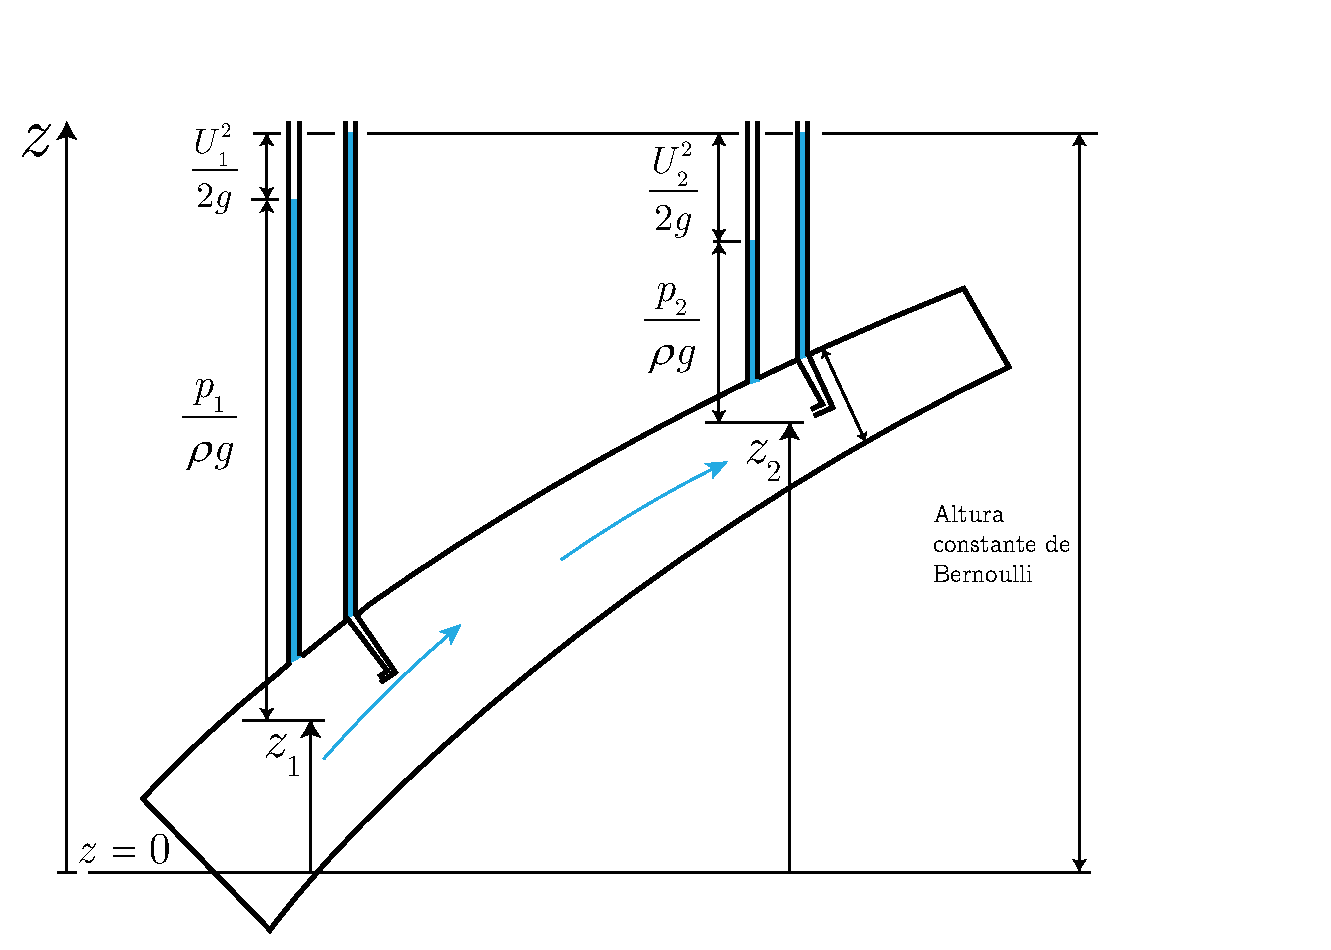
\includegraphics[width=.5\textwidth]{fig/bernoullidiag.eps}
    \caption{Visualización de la ecuación de Bernoulli \underline{sin pérdidas} en un caño que se va achicando en sección. Notar la diferencia entre la medida de un piezómetro y un tubo de pitot (ver condición de no-deslizamiento).}
    \label{fig:diagramaBernoulli}
\end{figure}
\subsection{Bernoulli generalizada}
Bernoulli con pérdidas, tomando en cuenta el perfil de velocidades (flujo bidimensional), siempre planteando el punto 1 del volumen de control ``aguas arriba":
\begin{equation}\label{eq:bernoulliPerdidas}
    \overbrace{\frac{\dot{W}}{gQ\rho}}^{I}+\overbrace{\frac{p_1}{g\rho}}^{II}+\overbrace{\frac{\alpha_1 U_1^2}{2g}}^{III}+\overbrace{z_1}^{IV}=\frac{p_2}{g\rho}+\frac{\alpha_2 U_2^2}{2g}+z_2+\overbrace{h_p}^{V}
\end{equation}
\begin{itemize}
    \item[I.] Altura relacionada al trabajo $\dot{W}$ hecho por bomba(s) o reacción química. Es igual a la altura $H_{\RM{B}}$ referida en el próxima sección
    \item[II.] Altura relacionada a la presión estática
    \item[III.] Altura relacionada a la presión dinámica
    \item[IV.] Altura de referencia del punto 1 del volumen de control tomado
    \item[V.] Altura de las pérdidas
\end{itemize}
donde $Q$ [\si{\meter \cubed \per \second}] es el caudal y $h_p$ es la altura de las pérdidas entre los puntos $1$ y $2$. 
\subsubsection*{Factor de correción a la energía $\alpha$}
El número $\alpha_1$ es un factor de corrección para la energía cinética que relaciona la velocidad media $U_1$ con el perfil de velocidades en el tubo. En régimen laminar $\alpha_{\textrm{laminar}}=2,0$. Para flujo turbulento con perfil del tipo
\[
U(r)=U_0 \left(1-\frac{r}{R}\right)^{m}
\]
donde $m$ suele variar entre $\frac{1}{5}$ y $\frac{1}{9}$
\[
\alpha_{\textrm{turb.}}=\frac{(1+m)^3(2+m)^3}{4(1+3m)(2+3m)}
\]
en general se suele tomar $\alpha_{\textrm{turb.}}=1,0$ para análisis elemental ya que este varía entre $\alpha_{\textrm{turb.}}\approx 1,04\mhyph1,11$.

\subsubsection*{Altura de las pérdidas $h_p$}
\vspace{-.75cm}
\begin{equation} \label{eq:alturaPerdidas}
    h_p=\overbrace{\sum^{n_L}_\iota \frac{U_\iota}{2g} \cdot \bigg(f_\iota\frac{L_\iota}{D_\iota}\bigg)}^{I}+\overbrace{\sum^{n_K}_\kappa \frac{U_\kappa}{2g} \cdot \big(K_\kappa\big)}^{II}
\end{equation}
donde $f$ es el \textit{factor de fricción de Darcy} y está en función del diámetro de la tubería ($D$), la rugosidad de las paredes de la tubería ($\epsilon$) y el número de Reynolds ($\Reynolds_D$). $L$ es la longitud del trayecto con pérdidas distribuidas. El término asociado con las perdidas \underline{no} va acompañado con un factor de corrección $\alpha$. 
\begin{itemize}
    \item[I.] Término relacionado a las pérdidas distribuidas
    \vspace{-.2cm}
    \item[II.] Término relacionado a las pérdidas localizadas
\end{itemize}
La razón por la cual se expresan las pérdidas como una sumatoria es porque a lo largo del trayecto el tubo puede cambiar de diámetro, y por lo tanto, también de velocidad. Cada pérdida tiene que ser calculada con su velocidad correspondiente, sea distribuida o localizada.

%%%%%%%%%%%%
%% BOMBAS %%
%%%%%%%%%%%%
\subsection{Instalaciones con bombas}

Cada bomba centrifuga tiene su curva característica caudal $Q$ versus altura $H_{\RM{B}}$. Esta se puede aproximar con una cuadrática de aspecto
\begin{equation}
    H_{\RM{B}} = A_{\RM{B}}+B_{\RM{B}} Q^2
\end{equation}
donde $A_{\RM{B}}$ y $B_{\RM{B}}$ son constantes que se pueden obtener del fabricante.

Un ingeniero suele estar interesado en si es apta una bomba para una instalación. Para que lo sea se tiene que verificar:
\begin{itemize}
    \item Existe una intersección de la curva de demanda (curva del sistema) con la curva de la bomba $H_{\RM{B}} = H_{\RM{S}}$
    \item No hay cavitación en ningún punto de la instalación
\end{itemize}
luego se podría verificar si el caudal que circula es suficiente para refrigerar la bomba correctamente o si se requiere más caudal para los propósitos del sistema.

La curva del sistema se obtiene planteando Bernoulli entre el punto de aspiración y de descarga.

\[
H_{\RM{S}}+\frac{p_a}{g\rho}+\frac{\alpha_aU_a^2}{2g}+z_a =\frac{p_d}{g\rho}+\frac{\alpha_d U_d^2}{2g}+z_d+h_p
\]
aquí tenemos el caudal camuflado en el término de la velocidad. Despejando y sabiendo que $U^2=\frac{Q^2}{(\pi D^2/4)^2}$

\begin{equation}
H_{\RM{S}} = A_{\RM{S}}+B_{\RM{S}}Q^2
\end{equation}
donde
\begin{gather*}
A_{\RM{S}} = \frac{p_d-p_a}{g\rho}+z_d-z_a \\
B_{\RM{S}} = \frac{8\alpha_d}{\pi^2gD_d^4}-\frac{8\alpha_a}{\pi^2gD_a^4}+\sum_k^n\frac{8}{\pi^2gD_k^4}\cdot\left(f_k\frac{L_k}{D_k}+K_k \right)
\end{gather*}
\newcommand{\Qstar}{{Q^{*}}}

Igualando $H_{\RM{B}}$ a $H_{\RM{S}}$ se obtiene el caudal que circularía si se instalara la bomba. Este caudal se suele escribir como $\Qstar$.\footnote{Aquí se agruparon las sumas de \eqref{eq:alturaPerdidas} para más claridad.}

\subsubsection*{El ANPA}
El \textbf{ANPA} (NPSH en inglés) es la Altura Neta Positiva de Aspiración. Es dada por el fabricante de la bomba e indica la caída de presión, en metros de columna de agua, entre la entrada de la bomba y la aspa en el interior. Se usa para verificar que no se produzca el fenómeno de la cavitación dentro de la bomba, pues esta puede ocasionar daños severos. Si no se cumple la siguiente igualdad hay peligro de cavitación:

\begin{equation} \label{eq:ANPA}
    \frac{p_{\entrada}}{\rho g} - ANPA - M_s > \frac{p_v(T)}{\rho g}
\end{equation}
donde $p_\entrada$ es la presión a la entrada de la bomba, $M_s$ es el margen de seguridad\footnote{Puede tomarse como 5 metros.} y $p_v(T)$ es la presión de vapor del liquido bombeado, el cual depende de la temperatura. 

Atento a los siguientes casos que comprometen la bomba:
\begin{itemize}
    \item Pérdidas altas en aspiración
    \begin{itemize}
        \item Tuberías angostas en aspiración
        \item Válvulas/filtros en aspiración
    \end{itemize}
    \item Bomba elevada sobre el nivel del fluido aspirado
\end{itemize}
\subsection{Turbulencia en caños}
Un lector ávido tal vez recuerde que $f$ está en función de $\Reynolds_D$. Esto no es un problema \textit{demasiado} grave en régimen laminar pues $f_{\textrm{laminar}}=\frac{64}{\Reynolds}$. En régimen turbulento sobran problemas numéricos...  Iterando sobre diferentes valores de $Q$ se obtienen valores de $\Reynolds_D$ y $f$ con la siguiente ecuación
\begin{equation} \label{eq:darcyExact}
    \frac{1}{\sqrt{f}}=-2\log \left[ \frac{\epsilon/D}{3,7}+\frac{2,51}{\Reynolds_D \sqrt{f}} \right]
\end{equation}
si uno no tiene ganas de resolver dado problema numérico puede usar una aproximación:
\[
\frac{1}{\sqrt{f}}\approx -1,8\log \left[ \left(\frac{\epsilon/D}{3,7}\right)^{1,11}+\frac{6,9}{\Reynolds_D}\right]
\]
también se tienen diversos diagramas de Moody a disposición del ingeniero (Ver figura \ref{fig:moodydiagram}).

Para hallar $\Qstar$ en régimen turbulento es necesario iterar para reducir el error cometido por no tener la solución exacta a \eqref{eq:darcyExact}. Los pasos a seguir son:

\begin{enumerate}
	\item[0.] Antes de comenzar la iteración se estima el caudal $\Qstar$ que podría estar circulando
	\setcounter{enumi}{0}
	\item Con el caudal se obtiene $f_{n}$ del diagrama de Moody o con la aproximación \label{enum:beginIteration}
	\item Se calcula $B_S$ con $f_{n}$ y se resuelve $H_S=H_B$ para obtener el caudal corregido 
	\item Se contrastan $f_{n}$ y el factor de fricción para el caudal corregido $f_{n+1}$ de tal forma que el error sea menor a 10\% para aplicaciones generales. Error $=\frac{f_{n+1}-f_{n}}{f_{n+1}}$
	\item Si no se verifica el error se repiten los pasos desde el paso \ref{enum:beginIteration} tal que $f_n=f_{n+1}$
	\item Se verifica la cavitación en el punto más comprometido de la instalación
\end{enumerate}

\begin{figure}[htb!]
    \centering
    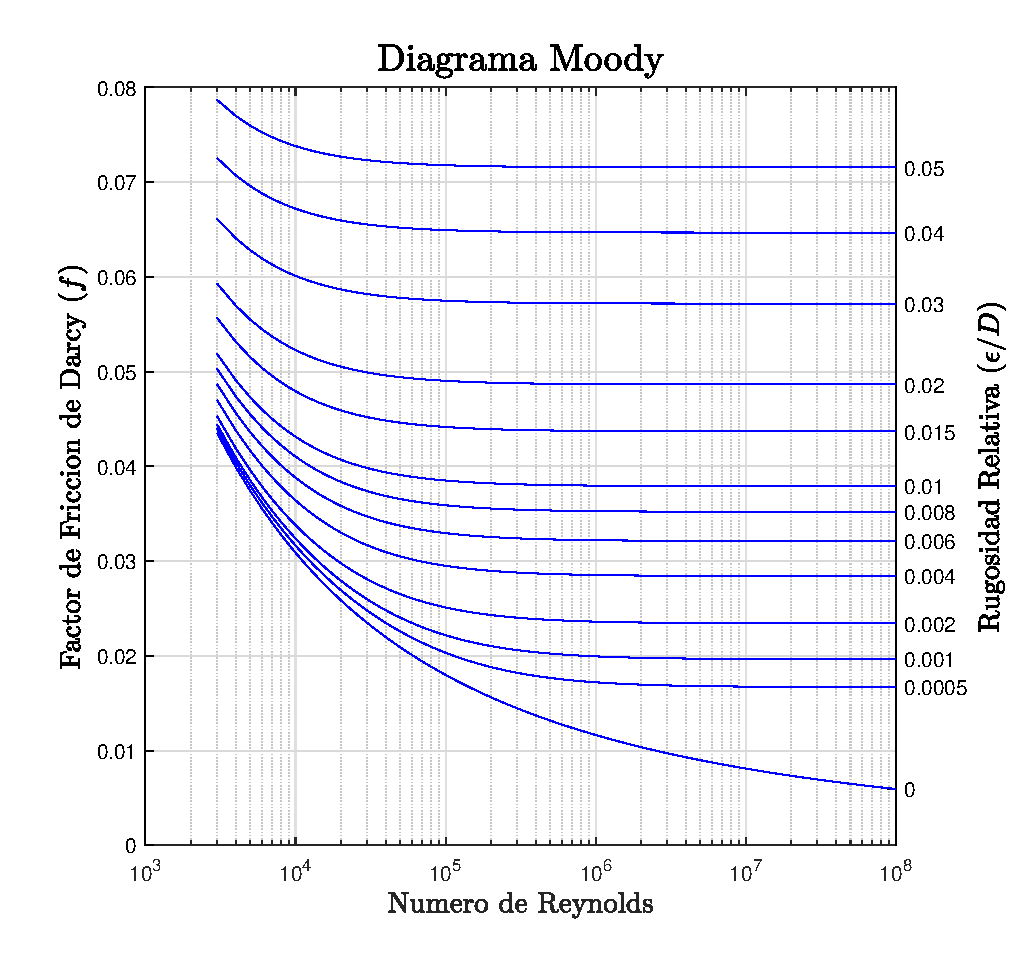
\includegraphics[width=0.475\textwidth]{fig/moodydiag.eps}
    \caption{Ecuación \ref{eq:darcyExact} graficada y resuelta numéricamente en \Matlab. Observe como a grandes Reynolds $f$ es constante para una dada rugosidad relativa.}
    \label{fig:moodydiagram}
\end{figure}

%%%%%%%%%%%%%%%%
%% SEMEJANZA  %%
%%%%%%%%%%%%%%%%

\section{Análisis dimensional}
Difiere de otros métodos de análisis por ser una forma de agrupar variables para dar un número adimensional. Estos números adimensionales rigen una variada estirpe de fenómenos físicos, como por ejemplo el número de Reynolds $\Reynolds$ (Ver tabla al comienzo del texto para más ejemplos). Las 7 \textbf{dimensiones base} son:
\begin{itemize}
    \item[$L$] Longitud
    \item[$M$] Masa
    \item[$T$] Tiempo
    \item[$\Theta$] Temperatura
    \item[$I$] Corriente eléctrica
    \item[$N$] Cantidad de substancia (mole)
    \item[$J$] Intensidad de luminosidad
\end{itemize}

En general se van a tratar problemas mecánicos ($LMT$) y termo-mecánicos ($LMT\Theta$).

\subsection{Teorema Pi de Buckingham}
 
 Para determinar el número de grupos adimensionales independientes que rigen un fenómeno físico se puede usar el teorema $\Pi$ de Buckingham. Según el teorema, el número de grupos adimensionales $j$ que se pueden formar para describir el problema es dado por
 \[
 j=n-m
 \]
 donde $n$ es el número de variables elegidos para describir el problema (viscosidad [$\mu$], longitud característica [$L,D,\ell$], conductividad térmica [$k$], etc.) y donde $m$ es igual a la cantidad de ecuaciones \textbf{independientes} formadas igualando los exponentes de cada dimensión base a cero (siempre menor o igual a la cantidad de dimensiones base) \citep{kreith2011principles}. 
 
 Para que un sistema sea \textit{completamente semejante} a otro tiene que cumplir con:
 \begin{itemize}
 	\item Semejanza Geométrica
 	\item Semejanza Cinemática
 	\item Semejanza Dinámica
 \end{itemize}
 
 \subsection{Ejemplo}
  En 1950 Sir Goffrey Taylor, un matemático británico, publica un artículo sobre análisis dimensional en el cual incluye un cálculo de la energía liberada de la primer bomba atómica ensayada en 1945 usando el teorema Pi de Buckingham. Taylor se basa en un video de la explosión que marcaba el tiempo desde detonación y una escala. 
  
  \begin{figure}[thb!]
  	\centering
  	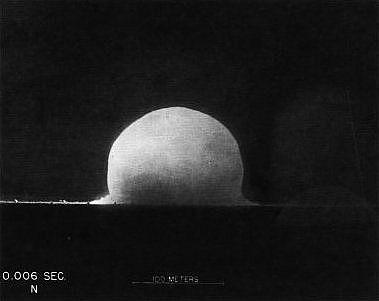
\includegraphics[width=0.9\linewidth]{fig/trinity1.jpg}
  	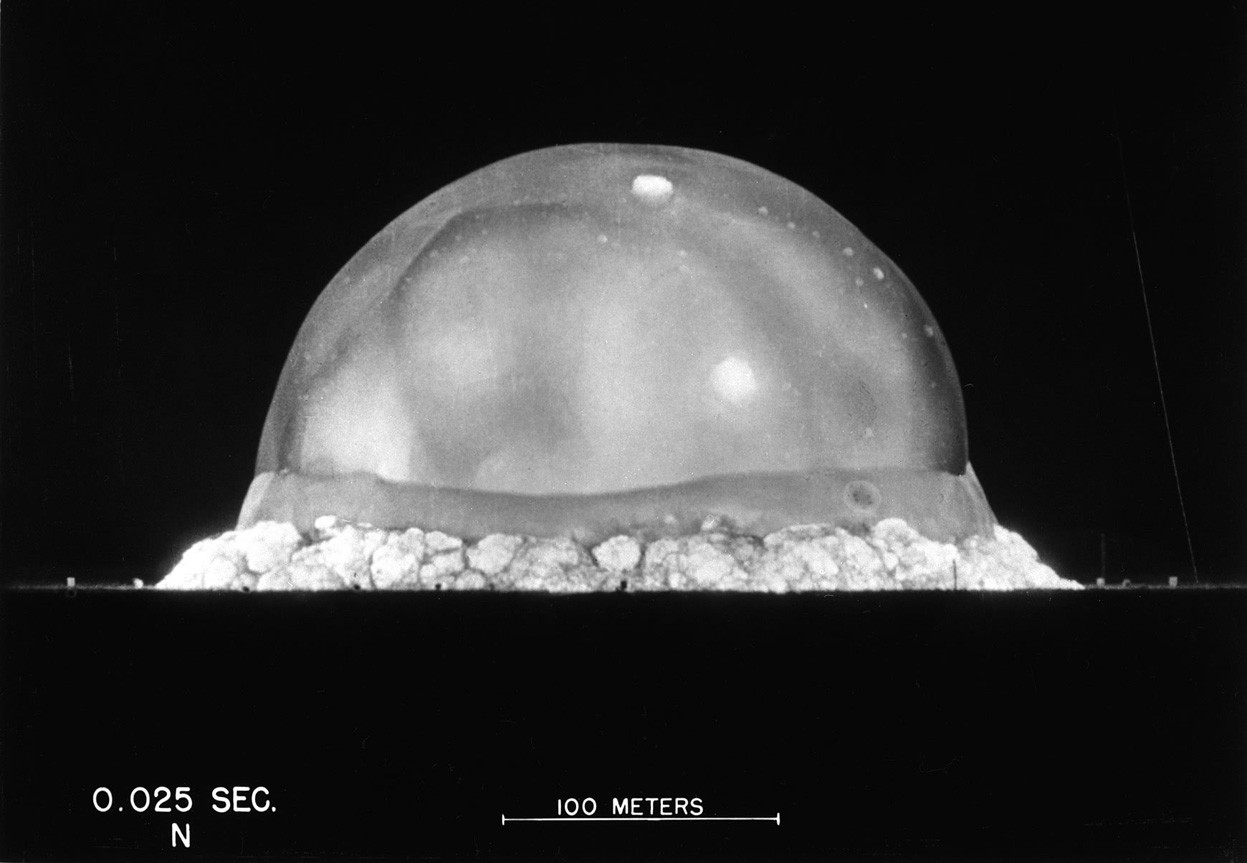
\includegraphics[width=0.9\linewidth]{fig/trinity2.jpg}
  	\caption{Onda de choque del primer ensayo de una bomba atómica denominado \textit{Trinity Test} [1945]. }
  	\label{fig:trinity}
  \end{figure}
 
 Se plantea que la energía liberada $E$ está en función de la densidad del medio $\rho$, el radio de la onda de choque $r$, y el tiempo $t$ desde la detonación, en total, 4 variables $n=4$. Se desprecian la viscosidad y la presión interna de la explosión
 
\begin{table}[htb!]
	\centering
	\begin{tabular}{l||l|lll}
		& $E$ & $t$ & $r$ & $\rho$ \\ \hline
		$L$ & 2   & 0   & 1   & -3     \\ \hline
		$M$ & 1   & 0   & 0   & 1      \\ \hline
		$T$ & -2  & 1   & 0   & 0     
	\end{tabular}
\end{table}
El sistema es independiente, entonces $m=3$. Según el teorema Pi de Buckingham, se puede formar un grupo adimensional $\Pi_1 = t^\alpha r^\beta \rho^\gamma E^\delta $
 
\begin{equation*}
	E = t^\alpha r^\beta \rho^\gamma = \begin{cases}
	L:& 2=\beta - 3\rho \\
	M:& 1= \rho \\
	T:& -2 = \gamma
	\end{cases}  
\end{equation*}

Resolviendo el sistema de arriba llegamos a que 
\[E = \frac{\rho r^{5}}{t^{2}} \]
Las dos imágenes en la figura \ref{fig:trinity} son para una explosión de $22$ kT de TNT, equivalente a aproximadamente $10 ^{14}$ joules. Con que certeza se puede calcular la energía de la \textit{Trinity Test} usando el teorema Pi? 







%% ENERGY EQUATIONS of LOCALITY

%%%%%%%%%%%%%%%%%%%%%%%%%%%%%%%%%%%%%%%%%%%%%
\section{Ecuaciones básicas locales}
\textit{En este texto las ecuaciones locales se obtendrán partiendo de la forma integral de la derivada material.}

Las leyes básicas de la física son:
\begin{itemize}
    \item Conservación de la masa
    \item Conservación de la cantidad de movimiento
    \item Conservación de la energía
    \item Conservación de las especies químicas
    \item Ecuación de estados 
\end{itemize}
Se puede aplicar TTR a toda propiedad extensiva de un sistema. 
\subsection{Derivada material}
Un medio fluido puede ser descrito de forma Lagrangiana o Euleriana.
\begin{itemize}
	\item \textbf{Lagrangiana.} Un tratamiento \textit{material} del fluido y se trabaja con funciones.
	\item \textbf{Euleriana.} Se trabaja con campos para describir el fluido
\end{itemize} 


Imagine que se tiene un flujo que puede ser descrito por un campo de velocidades $U_j(x,y,z,t)$. Si a uno le interesa puede obtener el cambio de velocidad en $x$ en $t$, obteniendo así: $\spartial{U_x}{t}$. Parecería ser que obtuvimos una aceleración por la forma pero no es el caso. Como bien sabemos, la aceleración está ligada a un objeto con masa, en este caso, las partículas del fluido cuya aceleración es influenciada por la derivada local ($\spartial{U_x}{t}$) y la \textit{convectiva} o \textit{advectiva} ($U_x\spartial{U_x}{x}+U_y\spartial{U_x}{y}+U_z\spartial{U_x}{z}$).

Se define entonces el operador \textit{derivada material}
\begin{equation}
\lim_{\Delta t \rightarrow 0} \frac{B(\vec{x}+\Delta \vec{x};t+\Delta t) - B(\vec{x};t)}{\Delta t} = \frac{\Di B}{\Di t}
\end{equation}

\[
\frac{\Di [\;]}{\Di t}=\spartial{[\;]}{t}+u_i\spartial{[\;]}{x_i}
\]
 El componente $j$ de la aceleración que un elemento de un fluido experimenta en un punto $x_i$ en el campo $U_j(x_i,t)$ está dada por
\[
a_j=\frac{\Di U_j}{\Di t}=\spartial{U_j}{t}+U_i\spartial{U_j}{x_i}
\]

\subsection{Teorema de transporte de Reynolds}

La ecuación general de Reynolds para una propiedad \textit{extensiva} $N$ del fluido en el volumen del control $V$ viene dada por la derivada material expresada en forma integral:

\begin{equation} \label{eq:TTRgeneral}
    \frac{\Di N_{\textrm{VC}}}{\Di t} \equiv \spartial{    }{t} \int_{V} \rho \eta \di \vol + \int_{S}\rho \eta u_i n_i \di \sur
\end{equation}
donde $\eta$ es la propiedad \textit{intensiva} del fluido\footnote{Intensiva son todas las propiedades que no dependen de la masa o el volumen de un cuerpo como densidad, punto de ebullición, presión, etc.} por unidad de masa del fluido y $n_i$ es el vector normal a la superficie del volumen de control.

Si se emplea el teorema de la divergencia de Gauss se puede pasar el integral de superficie a uno de volumen y agrupar. El teorema de Gauss escrito tensorialmente establece
\[
\int_{S}  N_k n_k \di \sur = \int_{V} \partial_k N_k \di \vol
\]
aplicando el teorema de la divergencia, nos queda el TTR de la forma

\begin{equation} \label{eq:TTRdivergence}
\frac{\Di N}{\Di t} \equiv \int_{V} \spartial{\rho \eta}{t}\di \vol +\int_V \spartial{\eta_k}{x_k} \di \vol=\int_V\left(\spartial{\rho \eta}{t} + \spartial{\eta_k}{x_k}\right)\di \vol
\end{equation}

La ecuación \ref{eq:TTRdivergence} resulta poco útil al momento de querer calcular lo que está adentro del integrando. En el caso de que se conserve la cantidad $N$ (como podría ocurrir en régimen estacionario) ocurre que $\frac{\Di N}{\Di t}=0$. Como $V$ está definido como un volumen arbitrario lo que está adentro del integrando debe ser cero: $\spartial{\rho \eta}{t} = - \spartial{\eta_k}{x_k}$, cuando se conserva $N$.

\subsection{Compresibilidad}
A partir del Teorema de Transporte de Reynolds (TTR) para masa en un volumen de control $V$
$$\frac{\Di M}{\Di t}\equiv\frac{\di }{\di t}\int_V \rho\di \vol +\int_S \rho u_k n_k \di \sur $$
que con la identidad de divergencia se tiene
$$\frac{\Di M}{\Di t} \equiv \int_V \left( \spartial{\rho}{t}+\spartial{\rho u_i}{x_i} \right) \di \vol $$
para un volumen de un fluido en \textbf{régimen estacionario} se tiene que $\frac{\Di M}{\Di t}=0$. A raiz de esto se puede decir que lo que está adentro del integrando es igual a cero:
\begin{equation} \label{eq:continuidad}
    \spartial{\rho}{t} +\spartial{\rho u_i}{x_i}=0
\end{equation}
Se le suele llamar ecuación de conservación de masa o simplemente \emph{continuidad} a la expresión \ref{eq:continuidad}.\par

Con la regla de la cadena, la divergencia se expande y se pueden agrupar términos tal que
\begin{equation} \label{eq:compresibilidad}
\frac{\Di \rho}{\Di t}+\rho \spartial{u_i}{x_i} =0
\end{equation}
la cual establece una definición mas precisa de la compresibilidad \citep{vieytes2018filminas}.

Sí se tiene un flujo de densidad constante en todo su punto (incompresible) se llega a que la divergencia de la velocidad es cero.
\begin{equation} \label{eq:incompresible}
    \diverg u_i =\spartial{u_i}{x_i}=0
\end{equation}


\subsection{Newton o TTR de cantidad de movimiento}
\label{sec:NewtonTTR}
\begin{align*}\numberthis{}
\overbrace{\frac{\Di \textbf{p}_j}{\Di t}}^{\textrm{I}}\equiv \overbrace{\frac{\di}{\di t}\int_V \rho u_j \di \vol}^{\textrm{II}} +\overbrace{\int_{S} \rho u_{j} u_{k} n_{k} \di \sur }^{\textrm{III}}& \\
   = \underbrace{\int_V B_j \di\vol}_{\textrm{IV}} +& \underbrace{\int_S \sigma_{ij}n_i \di \sur}_{\textrm{V}} 
\end{align*}  
Donde $B_{j}$ son las fuerzas por unidad de volumen o fuerzas volumétricas. $\sigma_{ij}$ es el tensor de tensiones. Los términos IV y V juntos son $\sum F_j$, la suma de las fuerzas externas sobre el volumen de control 
\begin{itemize}
    \item[I.] Derivada material de la componente $j$ de la cantidad de movimiento adentro del volumen de control $V$
    \item[II.] Cambio temporal del componente $j$ de la cantidad de movimiento en el interior de $V$
    \item[III.] Flujos de cantidad de movimiento entrantes y salientes por unidad tiempo en dirección $j$ sumados sobre la superficie entera del VC $S$
    \item[IV.] Componente $j$ de la fuerzas actuando por unidad de masa
    \item[V.] Componente $j$ de la suma de todas las fuerzas externas que actúan sobre la superficie del volumen de control $S$
\end{itemize}

Operando de forma similar a lo visto anteriormente

\begin{equation} \label{eq:ttrpTransitorio}
\spartial{\rho u_j}{t}+\spartial{\rho u_i u_j}{x_i}=B_j+\spartial{\sigma_{ij}}{x_i}
\end{equation}
Esta ecuación se puede trabajar con continuidad en régimen estacionario (\ref{eq:continuidad}) para llegar a una forma mas simple:
\begin{equation} \label{eq:ttrp}
    \rho \spartial{u_j}{t} +\rho u_i \spartial{u_j}{x_i}=B_j+\spartial{\sigma_{ij}}{x_i}
\end{equation}

El ultimo termino de la ecuación \ref{eq:ttrp} nos complica al querer modelar la realidad. No tenemos forma de meternos a un fluido para medir el estado de deformaciones y así obtener las tensiones. Se tiene que trabajar la ecuación un poco mas...
\begin{mdframed}
La ecuación de Euler es valida para flujos invíscidos ($\mu=\lambda=0$):
\begin{equation} \label{eq:eulerDiff}
    \spartial{u_j}{t}+u_i\spartial{u_j}{x_i}+\frac{1}{\rho}\spartial{p}{x_j}=\frac{B_j}{\rho}=b_j
\end{equation}
Donde $b_i$ son las fuerzas por unidad de masa.
\end{mdframed}
\subsection[Como reescribir los esfuerzos]{Como tratar $\sigma_{ij}$}
%\subsection{Como reescribir los esfuerzos }
Separamos $\sigma_{ij}$ en dos, su parte ``equilibrada'' isótropa y su parte desviadora similar a lo visto en la sección \ref{sec:presionmecanica}. 
\begin{equation}\label{eq:sigma1}
\sigma_{ij}=-p \delta_{ij} +S_{ij}
\end{equation}


$S_{ij}$ representa cuanto se desvía $\sigma_{ij}$ de las condiciones necesarias para el equilibrio y se lo suele llamar el tensor desviador. $\pe$ es la presión de equilibrio/termodinámica/hidrostática.

\[S_{ij}=A_{ijkl}\spartial{u_k}{x_l} \]

\begin{itemize}
\item Sí el fluido es \textbf{Newtoniano} entonces nos queda que $A_{ijkl}$ es \textbf{lineal} y depende del estado termodinámico.

\item Como $S_{ij}$ es \textbf{simétrico} entonces $A_{ijkl}$ es simétrico también \textbf{sobre los índices }$ij$. 

\item Para \textbf{fluidos simples} $A_{ijkl}$ es un tensor isótropo y se puede escribir de la siguiente manera donde $\mu=\mu^\prime$ por la simetría de $A_{ijkl}$ sobre $ij$.
\end{itemize}
\begin{equation} \label{eq:Aijklexpanded}
    A_{ijkl}=\lambda\delta_{ij}\delta_{kl} +\mu\delta_{ik}\delta_{jl}+\mu^\prime \delta_{il}\delta_{jk}=\lambda\delta_{ij}\delta_{kl} +2\mu\delta_{ik}\delta_{jl}
\end{equation}

\begin{itemize}
\item Basándonos en \ref{eq:Aijklexpanded} vemos que $A_{ijkl}$ es \textbf{simétrico sobre} $kl$
\end{itemize}
Mediante una descomposición falopa, el tensor gradiente de velocidades se reescribe en su parte simétrica $e$ y antisimétrica $\xi$. Recordemos que la contracción de un tensor simétrico y uno antisimétrico es $0$.
$$\spartial{u_k}{x_l}=e_{kl}+\xi_{kl}$$
$$A_{ijkl}\spartial{u_k}{x_l}=A_{ijkl}e_{kl}+\cancelto{0}{A_{ijkl}\xi_{kl}} $$

$$\therefore S_{ij}= A_{ijkl}e_{kl}=\lambda\delta_{ij}\delta_{kl}e_{kl} +2\mu\delta_{ik}\delta_{jl}e_{kl}$$
\begin{equation}
    S_{ij}=2\mu e_{ij}+\lambda e_{kk} \delta_{ij}
\end{equation}
$\mu$ es la viscosidad al corte o \emph{primera viscosidad}, $\lambda$ es la viscosidad de volumen o \emph{segunda viscosidad}. Ambas dependen del estado termodinámico del fluido. La igualdad $e_{kk}=\spartial{u_k}{x_k}$ es valida, en cambio $e_{ij}=\frac{1}{2}\left(\spartial{u_i}{x_j}+\spartial{u_j}{x_i}\right)$ ya que definimos el tensor desviador como el negativo de tau que se hablo en la sección \ref{sec:reologia}
\[
S_{ij}=-\tau_{ij}
\]

Por lo tanto, para un fluido Newtoniano tenemos:
\begin{equation}\label{eq:sigmanewt}
\sigma_{ij}=-p\delta_{ij}+\lambda e_{kk}\delta_{ij}+2\mu e_{ij} 
\end{equation}
%%%% NEW INCLUDE


% %%%
% Nos interesa la traza del tensor de desviaciones para definir la presión mecánica $p$ en función de la presión termodinámica
% $$ \textrm{tr}\;S_{ij}=S_{ii}=\left( 3\lambda +2\mu \right)e_{kk}$$
% \begin{equation}\label{eq:presionmec}
% p\equiv -\frac{1}{3}\sigma_{kk}=\pe-\left(\lambda +\frac{2}{3}\mu\right) e_{kk}
% \end{equation}
% usando \eqref{eq:presionmec} 

% \begin{equation} \label{eq:sigmamecanica}
% \sigma_{ij}=-\left[\pe -\left(\lambda+\frac{2}{3}\mu \right)e_{kk}\right]\delta_{ij} + \overbrace{2\mu \left(e_{ij}-\frac{1}{3}e_{kk}\delta_{ij}\right)}^{S_{ij}\textrm{}}
% \end{equation}


% La \textbf{hipótesis de Stokes} supone que $\pe=p \Rightarrow\lambda=-\frac{2}{3}\mu$. Nos queda entonces

% $$\sigma_{ij}=-\left(p+\frac{2}{3}\mu e_{kk} \right) \delta_{ij}+2\mu e_{ij} $$

\subsection{Navier--Stokes reducida}
Partimos de la ecuación de la conservación de momento local reescrita con $S_{ij}$ y la presión mecánica:
\begin{equation} \label{eq:NewtonSij}
    \frac{\Di \rho u_j}{\Di t}\equiv   \spartial{\rho u_j}{t}+\spartial{\rho u_i u_j}{x_i}=B_j-\spartial{p}{x_j}+\spartial{S_{ij}}{x_i}
\end{equation}

Consideremos ahora:
\begin{itemize}
\item Fluido Newtoniano
\item Fluido simple (isótropo)
\item Régimen estacionario
\end{itemize}
Estas hipótesis nos dan la ecuación de Navier--Stokes (\ref{eq:NS}) en su forma más generalizada para fluidos compresibles combinando \ref{eq:ttrp} y \ref{eq:sigmanewt}
\begin{mdframed}
\textbf{La ecuación de Navier--Stokes generalizada}
\begin{equation} \label{eq:NS}
     \rho \left( \spartial{u_j}{t}+u_i \spartial{u_j}{x_i}\right)=B_j-\spartial{p}{x_j}+2\spartial{\mu e_{ij}}{x_i}+\spartial{\lambda e_{kk} }{x_j}
\end{equation}
\end{mdframed}

Luego proponiendo unas cuantas hipotesis más:
\begin{itemize}
\item Hipotesis de Stokes $\pe=p\quad\Rightarrow\quad\lambda = -\frac{2}{3}\mu$
\end{itemize}
nos queda una formulación más aplicable, pero aún considerando flujos compresibles

\begin{equation}\label{eq:NS_stokesHipotesis}
     \rho \left( \spartial{u_j}{t}+u_i \spartial{u_j}{x_i}\right)=B_j-\spartial{\pe}{x_j}+2\spartial{\mu e_{ij}}{x_i}-\frac{2}{3}\spartial{\mu e_{kk}}{x_j}
\end{equation}

Si nos interesa el caso especial de un flujo incompresible e isotérmico se puede obtener la ecuación de Navier--Stokes reducida con dos hipótesis más:
\begin{itemize}
    \item Flujo isotérmico $\spartial{T}{x_j}=0$
    \item Incompresibilidad ($e_{kk}=0$)\footnote{Una consecuencia de incompresibilidad es que $\rho$ sea constante.}
\end{itemize}
Nos queda la ecuación de N--S reducida (\ref{eq:NSr})
\begin{mdframed}
\textbf{Navier--Stokes reducida.}\footnote{Dado que el flujo es isotérmico la viscosidad no depende de la posición.}
\begin{equation}\label{eq:NSr}
\rho \left( \spartial{u_j}{t} +u_i \spartial{u_j}{x_i}\right)=B_j-\spartial{\pe}{x_j} +\mu \spartial{^2 u_j}{x_i\partial x_i}
\end{equation}
\end{mdframed}



\subsection{Energía cinética}

\begin{equation}\label{eq:eCinetica}
\frac{\Di \ek}{\Di t}\equiv u_i b_i-\frac{1}{\rho}\spartial{(u_k p)}{x_k} +\frac{1}{\rho} \spartial{(u_i S_{ij})}{x_j}+\frac{1}{\rho} \frac{p\partial u_k}{\partial x_k}-S_{ij} \frac{\partial u_i}{\rho \partial x_j}
\end{equation}

El cambio de energía cinética en un fluido (\ref{eq:eCinetica}) viene dado por el trabajo realizado por unidad de tiempo por: las fuerzas por unidad de masa, la presión, y los esfuerzos cortantes. Los últimos dos sumandos representan la conversión \emph{reversible} de energía cinética en energía interna y la disipación \emph{irreversible} de energía por esfuerzos cortantes.
\subsection{Energía interna}
Se define $\et$ como la energía total del fluido.
\begin{equation}\label{eq:etotal}
    \dot{Q}-\dot{W}_\textrm{M}=\frac{\di }{\di t}\int_V \rho \et \di \vol +\int_S \rho \et u_j n_j \di \sur
\end{equation}

Donde $\dot{Q}$ es el calor que recibe el fluido por unidad de tiempo sea por las paredes por diferencia de temperatura o el calor generado en el seno del fluido por algún proceso (nuclear, química, disipación etc.), y $\dot{W}_\textrm{M}$ es la potencia intercambiada por el sistema (mecánica).


 La ecuación \ref{eq:Qk} describe la potencia entregada por las superficies al fluido. Recordemos que en el curso vamos a trabajar fluidos isótropos y por lo tanto $k_{ij}=-k \delta_{ij}$. Sabiendo la potencia entregada por unidad de superficie $q_i^{\prime \prime}=k_{ij}\spartial{T}{x_j}=-k\delta_{ij}\spartial{T}{x_j}$ 
\begin{equation}\label{eq:Qk}
    \dot{Q}_K=\int_S q_i^{\prime \prime} n_i \di \sur = -\int_S - k\delta_{ij}\spartial{T}{x_j}n_i \di \sur
\end{equation}
Lo que calculamos aquí es la potencia entregada por el fluido, por lo cual le va un signo menos adelante por convención (Calor recibido es positivo). El signo menos del termino $q_i^{\prime \prime} $ sale de la necesidad que el flujo de calor sea positivo cuando $\spartial{T}{x_j}$ es negativo (Calor fluye de mayor $T$ a menor $T$).


\begin{align*}
    \dot{Q}=\int_S k\spartial{T}{x_j} n_j \di \sur + \int_V \dot{q}_G \di \vol &=\\
    \int_V \bigg[ &\spartial{ }{x_j} \bigg( k   \spartial{T}{x_j} \bigg) + \dot{q}_G \bigg] \di \vol
\end{align*}
Ok:
\begin{equation} \label{eq:etotalreplace}
    \rho \frac{\Di \et}{\Di t}\equiv \spartial{}{x_j}\left(k\spartial{T}{x_j}\right) - \spartial{u_i p}{x_j}+\spartial{u_i S_{ij}}{x_j}+\rho u_i b_i+\dot{q}_G
\end{equation}
Entonces restando \ref{eq:eCinetica} y \ref{eq:etotalreplace} tenemos la ecuación de la energía interna \ref{eq:einterna}

\begin{equation} \label{eq:einterna}
    \rho \frac{\Di \textrm{e}}{\Di t}\equiv \spartial{}{x_j}\left( k\spartial{T}{x_j}\right) - p \spartial{u_j}{x_j} +\overbrace{S_{ij} \spartial{u_i}{x_j}}^{=\Phi \textrm{ (ver \eqref{eq:disipcartesianas})}}+\dot{q}_G
\end{equation}
\newcommand{\dstar}{\delta^{*}}
\section{Capa limite para placas planas}
Una placa plana inmersa en un fluido con velocidad relativa puede asemejarse a una lista variada de problemas de ingeniería desde aviones hasta intercambiadores de calor. El concepto de la capa límite es simplemente el interfaz virtual entre la zona donde dominan los efectos viscosos y la zona invíscida. 

Más precisamente:\textit{ La capa límite se dibuja como una linea donde la velocidad absoluta del flujo es 99\% de la velocidad del flujo ``en el infinito"{}}($U_\infty$).\footnote{Sobre la capa límite y toda la región inviscida se desprecia $\spartial{u}{y}$, el cual es proporcional al corte $\tau$.}

 Para el estudio de capas limites se parte de las hipótesis 
 
 \begin{itemize}
 	\item Flujo bidimensional $u_j = u \hat{\i} + v \hat{\j}$
 	\item Estacionario
 	\item Incompresible $ \spartial{u}{x}+\spartial{v}{y}=0$
 	\item Newtoniano  $\tau_{xy}=\mu \spartial{u}{y}$
 	\item Isotérmico $\spartial{T}{x}=\spartial{T}{y}=0$
 \end{itemize}

 Cantidad de movimiento:
\[
\rho\left(u\spartial{u}{x}+v\spartial{u}{y}\right)=\mu \dpartial{u}{y}-\spartial{p}{x}
\]

Solo se van a estudiar capas límites para Números de Reynolds altos $\Reynolds_\delta\gg 1$.\footnote{Un número adimensionales con un subíndice indica que longitud característica tomar. Por ejemplo: $\Reynolds_D= \frac{UD}{\nu}$}

\begin{figure}%[tb]
    \centering
    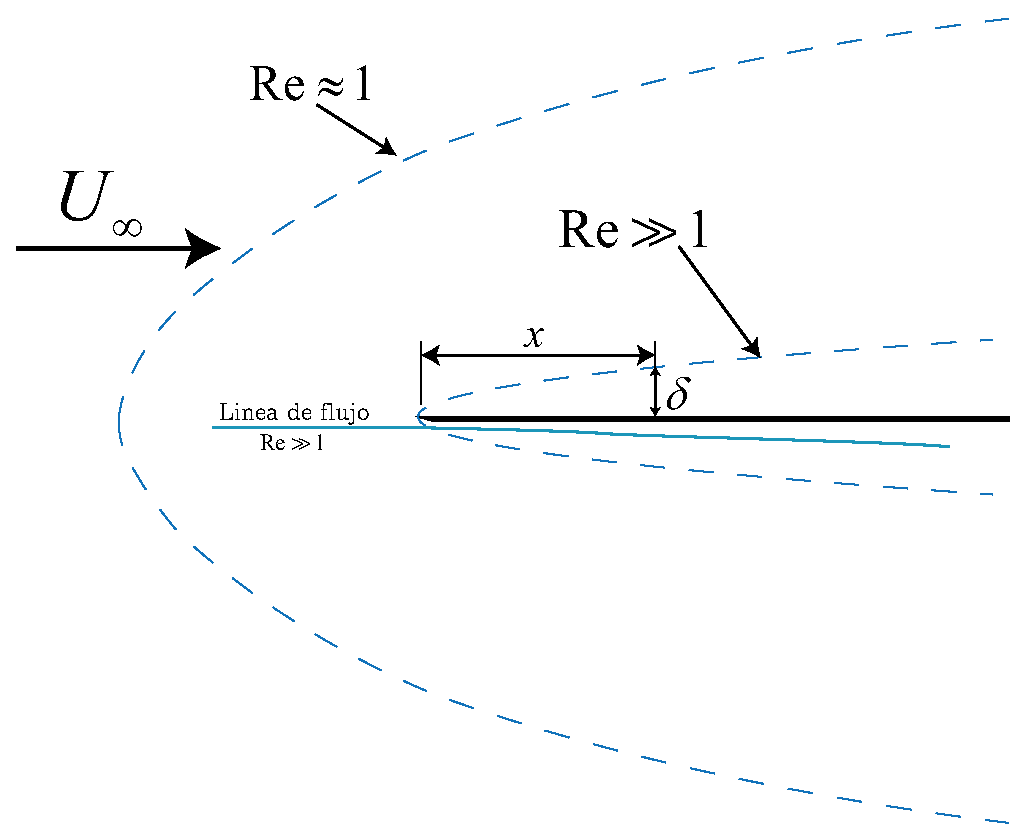
\includegraphics[width=0.47\textwidth]{fig/BL1.eps}
    \caption{Dos casos de capa límite muy diferente. Se va tratar capas límites con $\Reynolds_\delta \gg1$.}
    \label{fig:BLintro}
\end{figure}
\subsection{Solución analítica: Laminar}
En 1908 Paul Richard Heinrich Blasius, un físico alemán, desarrolla la teoría fundamental para el estudio de capa limites laminares sobre placas planas. Mediante un uso riguroso de la teoría de semejanza llega a la siguiente ecuación diferencial
\[
ff^{\prime\prime}+2f^{\prime\prime\prime}=0
\]
cuya solución (obtenida numéricamente con determinadas condiciones de borde) se denomina el perfil de velocidades de Blasius.
\[
\begin{array}{lll}
u(x,0)=0, & u(x,\delta)=U_\infty, & \tau|_{y=\delta} =0
\end{array}
\]

En base a este perfil de velocidades se desarrollan las siguientes relaciones \citep{durst2008fluid}:
\begin{equation}
    \delta=\frac{5,2x}{\sqrt{\Reynolds_x}}=5,2\sqrt{\frac{x\mu}{\rho U_\infty}}
\end{equation}

\begin{equation}
    \tau_s=\mu \left. \spartial{u}{y}\right|_{y=0}=0,332\,\mu\frac{U_\infty}{x}\sqrt{\Reynolds_x}=0,332\, U_\infty^{1,5}\sqrt{\frac{\rho}{x\mu}}
\end{equation}
donde $\tau_s$ es el la tensión de corte sobre la superficie de la placa. 

\begin{equation}
    c_f=\frac{\tau_s}{\rho U_\infty^2/2}=\frac{0,664}{\sqrt{\Reynolds_x}}
\end{equation}

\begin{equation}
    C_D=\bar{c}_f=\frac{1}{L}\int_0^Lc_f\di x=\frac{1,328}{\sqrt{\Reynolds_L}}
\end{equation}
donde $c_f$ es el coeficiente de fricción local sobre la placa y $C_D$ es el coeficiente de drag de la placa. La fuerza sobre la placa entera se puede entonces obtener dimensionalizando $C_D$ tal que
\[
F_D=\tfrac{1}{2}C_D \rho U_\infty A
\]

Las relaciones anteriores solo valen para régimen laminar. Se puede suponer que cualquier flujo $\Reynolds_L<\num{5e5}$ es laminar. Si el flujo no es perturbado y la superficie de la placa es pulida se puede demorar la transición a turbulento hasta $\Reynolds=\num{3e6}$ \citep{kreith2011principles}.

\subsubsection*{Efecto desviador de lineas de flujo}
A causa de la desaceleración del flujo cerca de la placa las lineas de flujo se tiene que desviar hacia afuera. 

Para el caso de la figura \ref{fig:displthickness} se tiene una placa plana con flujo $U_\infty$ incidente. En color (linea solida) esta dibujado la capa límite. Para hallar $\dstar$ se plantea un VC que siga la linea de flujo del punto $(x,y)=(0,h)$ hasta $(x,y)=(x_0,\delta)$. La incógnita es $h$ y se puede hallar planteando conservación de masa entre la entrada y salida del VC.

\begin{equation}
    \dstar \approx \frac{\delta}{3}  \qquad \textrm{donde}\qquad  \delta=h+\dstar
\end{equation}


\begin{figure}[htb!]
    \centering
    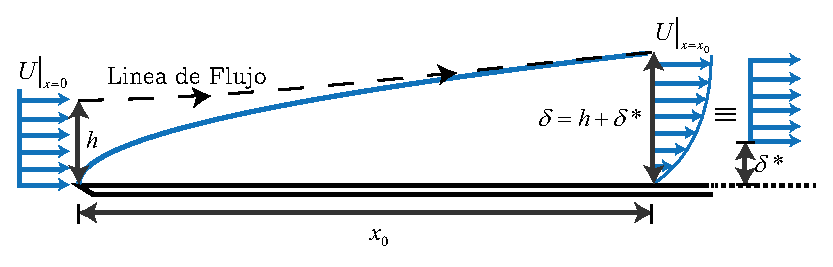
\includegraphics[width=0.47\textwidth]{fig/BLdispthick.eps}
    \caption{Efecto desviador de lineas de flujo y su efecto ``simulado"{} visto a la derecha.}
    \label{fig:displthickness}
\end{figure}

Demostración partiendo de conservación de caudal entre la entrada y salida donde $b$ es el ancho de la placa

\begin{gather*}
	\rho b \int^h_0 u(0;y)\di y = \rho b \int^{h+\dstar}_0 \!\!\!\!u(L;y)\di y \\
	\cancel{\rho b} h U_\infty =\cancel{\rho b}\int^{h+\dstar=\delta(x)}_0 \!\!\!\!\!\!\left[u(x;y)+U_\infty-U_\infty \right]\di y\\	
	\cancel{hU_\infty} = \int^{\delta(x)}_0 \!\!\!\!\!\!\left[u(x;y)-U_\infty \right]\di y+U_\infty (\cancel{h}+\dstar)
\end{gather*}
\begin{equation}
	\dstar = \int_0^{\delta(x)} \!\!\!\left(1-\frac{u(x;y)}{U_\infty} \right) \di y
\end{equation}


%%%%%%%%%%%%%%%%%%%%%%
%% TURBULENTO
%%%%%%%%%%%%%%%%%%%%%%

\subsection{Relación empírica: Turbulento}
En realidad una capa límite laminar siempre precede la turbulenta. Sin embargo el comienzo turbulencia se puede inducir sobre el filo de la placa usando alambre. Esto suele ser útil para aumentar la transferencia de calor y reducir el arrastre alto en régimen laminar.

Para flujo turbulento el espesor de capa límite no tiene solución exacta. Una relación empírica que se puede usar es la siguiente:
\begin{equation}
    \delta \approx \frac{0,22x}{\Reynolds_x^{\frac{1}{6}}}
\end{equation}

Prandtl sugiere usar (resultado final simplificado):
\[
c_f \approx 0,02\, \Reynolds_\delta^{-\frac{1}{6}} = 0,02\left(0,22 \Reynolds_x^{5/6}\right)^{-\frac{1}{6}}\approx \frac{0,026}{\Reynolds_x^{\frac{1}{7}}} 
\]

Otra formula que se puede usar \citep{kreith2011principles}:
\begin{equation}
    c_f=\frac{0,0576}{\Reynolds_x^{0,2}}
\end{equation}
No se pueden calcular los esfuerzos viscosos en la pared debido a la singularidad en $x=0$.

\[
\frac{\left\langle u \right\rangle}{U_\infty} = \left(\frac{y}{\delta} \right)^{\frac{1}{n}}, \quad n=7,8,9
\]
\subsubsection{Análisis capa mixta}

En el caso que demore la transisción a régimen turbulento se puede obtener la capa límite al final de la placa $\delta_L=\delta_{\mathrm{turb}}(L-x_0)$ despejando $x_0$ en
\[
\delta_\crit =\delta_{\mathrm{lam.}}(x_\crit) = \delta_{\mathrm{turb.}}(x_\crit-x_0) 
\]


\begin{figure}[htb!]
	\centering
	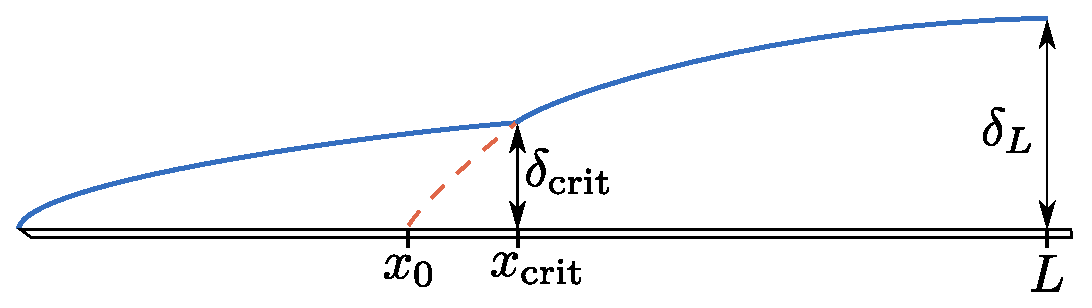
\includegraphics[width=0.48\textwidth]{fig/BLmixed.eps}
	\caption{Análisis de capa límite mixta.}
	\label{fig:BLmixed}
\end{figure}



\begin{figure}[htb!]
    \centering
    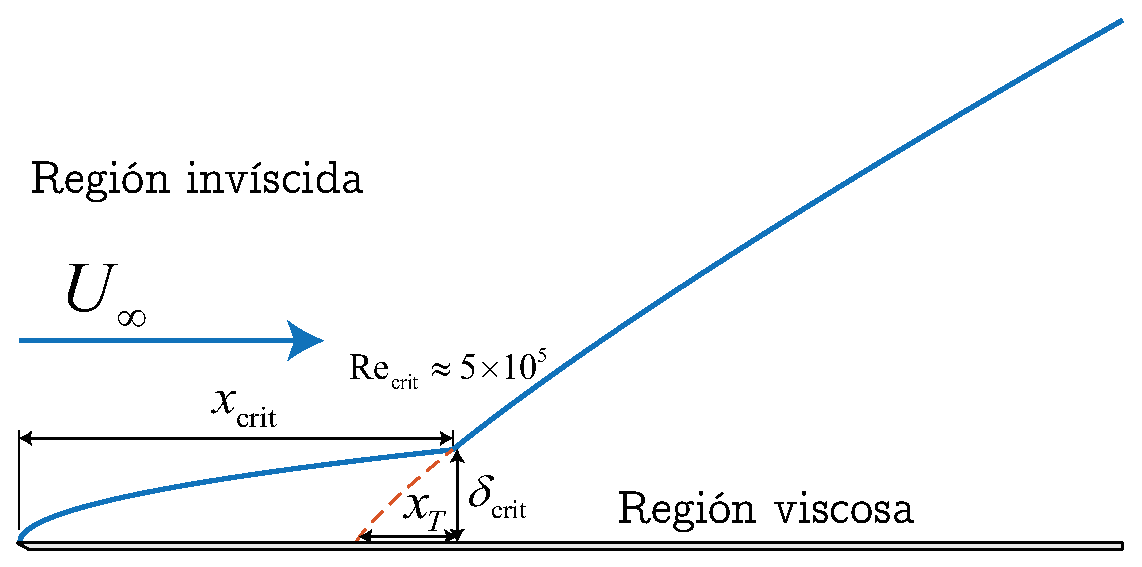
\includegraphics[width=0.48\textwidth]{fig/BLmixedejemplo.eps}
    \caption{Análisis de capa límite mixta de aire sobre una placa $L=10\si{\meter}$, $U_\infty=2\si{\meter\per\second}$. Resuelto en \Matlab.}
    \label{fig:BLmixedExample}
\end{figure}

\section{Flujo Potencial}
\subsection{Flujo potencial generalizado para 3-D}
La teoría de flujo potencial es útil para tratar problemas aerodinámicos e hidrodinámicos cuando se tiene un flujo invíscido (zona afuera de la capa límite) por su bajo costo computacional.

Hipótesis flujo potencial
\begin{itemize}
    \item Flujo invíscido
    \item Flujo irrotacional
    \item Régimen estacionario
\end{itemize}
Entonces existe una función potencial $\varphi$ tal que
\[
u_j = \partial_j \varphi \qquad \nabla^2\varphi = 0
\]
la segunda ecuación es equivalente a decir que el flujo es incompresible. La ecuación de Euler \eqref{eq:eulerDiff} es valida y se puede usar un Bernoulli de la forma
\begin{equation}
    \spartial{\varphi}{t}+\frac{p}{\rho}+\frac{||\partial_j \varphi||^2}{2}+gh=\textrm{const.}
\end{equation}
donde $h$ es la altura en el punto en cuestión, sea medido en $x,y$ o $z$.
\subsection{Flujo Potencial 2-D}



\section{Turbulencia}

\subsection{Cascada turbulenta}
Nos interesa el proceso de disipación y \textbf{por qué es inviable la simulación directa}. La energía que se transfiere de una escala a otra por una \textit{Eddy} está dada por 

\[
e_{\Lambda}=\frac{\mathscr{U}^2}{2 \mathscr{T}} \sim \mathscr{U}^3 \mathscr{L}^{-1}
\]
donde las cantidades $\{ \mathscr{U},\mathscr{L},\mathscr{T}\}$ son las cantidades características de velocidad, longitud y tiempo en la escala $\Lambda$.

La potencia disipada en los eddies será
\[
\Phi_\Lambda =\nu \left( \spartial{\mathscr{U}_i}{x_j} \right)^2 \sim \nu \mathscr{U}^2 \mathscr{L}^{-2}
\]
y la razón entre la energía específica y la potencia específica
\[
\Dscr_\Lambda = \frac{e_\Lambda}{\Phi_\Lambda} \sim \frac{\mathscr{U}^3 \mathscr{L}^{-1}}{\nu \mathscr{U}^2\mathscr{L}^{-2}}\sim \Reynolds_\Lambda
\]
Si $\Dscr_\Lambda$ es mayor que la unidad significa que en la escala $\Lambda$ hay poca disipación.

Definimos las tres escalas espaciales de la turbulencia

\begin{itemize}
    \item \textbf{Macroscópica:} $\Reynolds_L=\frac{UL}{\nu}\gg 1$ Caracterizada por baja disipación y carácter anisótropo. $\{ U,L,T\}$
    \item \textbf{Intermedia:} $\Reynolds_\ell = \frac{u\ell}{\nu}>1$ Baja disipación. $\{ u,\ell,\tau \}$
    \item \textbf{Microscópica o de altas frecuencias:} $\Reynolds_{\lambda_0}\sim 1$ Es la escala a la cual se produce la mayor parte de la disipación. Es un proceso isótropo. $\{ u_0,\lambda_0,\tau_0 \}$
\end{itemize}

Partiendo de una hipótesis que dice que la energía transferida es similar a toda escala $e_L\sim e_{\lambda_0}$ llegamos a que 
\[
U^3L^{-1}\sim u_0^3\lambda_0^{-1} \quad \Rightarrow\quad u_0\sim U \left(\frac{\lambda_0}{L} \right)^{\frac{1}{3}}
\]
por lo tanto tendremos
\[
\Reynolds_{\lambda_0}=\frac{u_0 \lambda_0}{\nu}\sim \Dscr_{\lambda_0}\sim U \left(\frac{\lambda_0}{L} \right)^{\frac{1}{3}} \frac{\lambda_0 L}{\nu L}=\Reynolds_L \left(\frac{\lambda_0}{L}\right)^{\frac{4}{3}}
\]
luego con la relación $\Reynolds_{\lambda_0}\sim 1 $ se obtiene que $\lambda_0\sim L \Reynolds_L^{-\frac{3}{4}}$ lo cual expresa la longitud característica a la cual sucede la mayor parte de la disipación. Lo importante que hay que llevarse de la expresión anterior es que a medida que aumenta el número de Reynolds $\lambda_0$ se vuelve diminuto. Si quisiéramos modelar estas estructuras para un problema macroscópico se necesitaría un poder de calculo que no existe ni el el supercomputador más polenta.

\subsection{Reynolds-Averaged Navier--Stokes}
Para el tratamiento de flujos turbulentos existe el metodo RANS que propone que las propiedades de un flujo turbulento pueden ser descompuestas en dos partes, el \textit{promedio} y la parte \textit{fluctuante}. 
\[
u_j=U_j+u^\prime_j
\]
la parte promediada $U_j$ es lentamente variable en el tiempo mientras que $u^\prime_j$ es rápidamente variable en el tiempo. 
\subsubsection*{Reglas del promediado en el tiempo}
El promedio temporal:
\[
\left< N_j\right>=\frac{1}{\Delta T}\int_t^{t+\Delta T}N_j\di t
\]

El álgebra:
\begin{equation}
\left<N +\alpha M \right>=\left< N\right> +\alpha \left< M \right>
\end{equation}
\[
\left< \int N \di x \right> = \int \left< N \right> \di x
\]

Si $N$ es una propiedad lentamente variable en el tiempo y $\eta$ una propiedad rápidamente variable en el tiempo, entonces:
\begin{gather}
\left< N\eta \right>=N \left< \eta \right> \\
\left< \int N \eta \di x\right> = N \int \left< \eta \right> \di x \\
\left< \spartial{(N\eta)}{s} \right> = \spartial{N}{s}\left< \eta \right> + N \spartial{\left< \eta \right>}{s}
\end{gather}
\subsubsection*{Promedio temporal}
Para el componente rapidamente variable en el tiempo se puede demostrar que su promedio temporal es nulo:
\begin{equation} \label{eq:promediotemporalCompRapidVar}
    \left<\eta_j^\prime\right>= 0
\end{equation}
dicha propiedad es importante tenerla en cuenta para todas las siguientes demostraciones.

Según continuidad \eqref{eq:continuidad}:
\[
\left< \spartial{u_k}{x_k}\right> =0
\]
llegamos a que 
\[
\spartial{U_k}{x_k} =0
\]

\subsubsection*{RANS}
\[
\spartial{u_j}{t}+u_k \spartial{u_j}{x_k}=-\frac{1}{\rho}\spartial{p}{x_j}+ \nu \dpartial{u_j}{x_k}+g_j
\]
podemos luego expandir el término velocidad en dos componentes
\begin{align*}
\left< \spartial{U_j}{t}+\spartial{u^\prime_j}{t}+U_k\spartial{U_j}{x_k}+U_k\spartial{u^\prime_j}{x_k}+u^\prime_k \spartial{U_j}{x_k}+u^\prime_k \spartial{u^\prime_j}{x_k} \right> &= \\
- \frac{1}{\rho}\left<\spartial{P}{x_j}+\spartial{p^\prime}{x_j} \right>+\nu\left< \dpartial{U_j}{x_k}+\dpartial{u^\prime_j}{x_k}+g_j\right>&
\end{align*}
operando 
\[
\spartial{U_j}{t}+U_k\spartial{U_j}{x_k}+\spartial{\left<u_j^\prime u_k^\prime\right>}{x_k}=-\frac{1}{\rho}\spartial{P}{x_j}+\nu \dpartial{U_j}{x_k}+g_j
\]%rst=Reynolds Stress tensor
de aqui en adelante se define el Tensor de tensiones de Reynolds $\rho\rst$ y se reescribe la ecuación anterior para obtener el RANS
\begin{align*}\numberthis \label{eq:RANS}
    \rho\left( \spartial{U_j}{t}\!+\!U_k\spartial{U_j}{x_k}\right)\! = \!-\spartial{P}{x_j}-\spartial{}{x_k}\left(\!-\mu \spartial{U_j}{x_k}\!+\!\rho\rst \right)\!+\!g_j
\end{align*}
%--------------------------------------------------------
%       Termina Refresh de Mecánica de Fluidos
%--------------------------------------------------------
 \setcounter{footnote}{0}
 
\section{Principios de transferencia de calor}
\subsection{Conducción de Calor}
\begin{equation} \label{eq:LaEcuacionBasica}
    q_k\propto A\frac{\di T}{\di x}\rightarrow q_k=-kA\frac{\di T}{\di X}
\end{equation}

El signo negativo en \ref{eq:LaEcuacionBasica} es por causa de la segunda ley de la termodinámica que nos dice que el calor fluye de un punto de mayor temperatura a uno de menor temperatura.

Temperatura uniforme cara plana.
$$q_k=-\frac{kA\Delta T}{L} $$
$$R_k=\frac{L}{Ak}$$

Analogía eléctrica:
$$V\sim T $$
$$I \sim \dot{q}_{\text{calor}}$$
$$R\sim\frac{1}{K}= \frac{1}{\bar{h}_cA}\sim \frac{L}{kA} $$
$$C=\frac{Q}{V}\sim c\cdot m \si{}$$
Conducción térmica
$$K_k=\frac{kA}{L}$$
La razón $k/L$ se le dice la conducción térmica unitaria. $L/k$ es la  resistencia térmica unitaria.

Aproximación lineal de conductividad térmica en función de la temperatura
$$k(T)=k_0(1+\beta_kT)$$ donde $\beta$ es un valor empírico.

Usando está ecuación se aproxima el calor intercambiado con un $k$ promedio.

$$q_k=\frac{k_{\textrm{prom}}A\Delta T}{L}$$

Ley de Fourier
$$ k=\frac{q_k/A}{|\di T/\di x|}$$

Dos mecanismos de transferencia de calor por conducción
\begin{itemize}
    \item Vibraciones de la estructura reticulada
    \item Transporte de electrones (el mas efectivo de los dos)
\end{itemize}
Los metales conducen calor de las dos formas mientras que los solidos no-metálicos solo conducen por vibraciones.
\subsection{Convección}
El mecanismo de transferencia de calor sigue siendo la conducción pero se hace la distinción porque la transferencia de calor está prácticamente determinada por el campo de
velocidad \citepalias{vieytes2018filminas}. 
$$q_c=-k_{\textrm{fluido}}A\left| \spartial{T}{y}\right|_{y=0} $$
$$q_c=\hcb A\Delta T $$
El coeficiente $h_c$ local esta dado por
$$ \di q_c=\hcb \di A(T_s-T_{\inf}) $$

$$\bar{h}_c=\frac{1}{A}\int_A\int h_c\di A$$
Conductividad térmica para transferencia de calor por convección:
$$K_c=\hcb A$$
Si el cuerpo está en presencia de una corriente externa la razón del número de Grashof sobre el cuadrado de Reynolds puede ser usada para determinar que modo de convección domina
\[
\frac{\Grashof}{\Reynolds^2}
\begin{cases}
\gg 1&\quad \!\textrm{Convección forzada despreciable} \\
\approx  1&\quad\! \textrm{Convección forz. y natural combinadas}\\ 
\ll 1 & \quad \! \textrm{Convección natural despreciable}
\end{cases}
\]
\subsection{Radiación}
Cuerpo negro $\varepsilon=1$. Cuerpo \textbf{rodeado completamente} por superficie a $T_2$ da $\fforma=1$. El factor de forma ($\fforma$) se tiene que tomar en cuenta cuando ambos cuerpos \textbf{no} son cuerpos negros y además tienen una relación geométrica.
$$q_r=A_1\fforma_{1\boldsymbol{-}2}\sigma(T_1^4-T_2^4) $$
$$K_r=\frac{A_1\fforma_{1\boldsymbol{-}2} \sigma(T_1^4-T_2^4)}{T_1-T_2}$$
Coeficiente de transferencia de calor por radiación: $\hrb=\frac{K_r}{A_1}$
\subsection{Termodinámica}
Primera ley de Termo. $e$ como energía especifica.
$$e\dot{m}_\textrm{entrada}+q+\dot{q}_G-(e\dot{m})_\textrm{out}-W_{\textrm{salida}}=\spartial{E}{t} $$

Para sistemas cerrados:
$$q+\dot{q}_G-W_{\textrm{salida}}=\spartial{E}{t}$$

Según la termodinámica, la entalpía se define como $h=\ei+\frac{p}{\rho}$

$$\frac{\Di h}{\Di t}=\frac{\Di \ei }{\Di t}+\frac{1}{\rho}\frac{\Di p}{\Di t}- \frac{p}{\rho^2} \frac{\Di \rho}{\Di t} $$
luego tenemos que 

\begin{equation}\label{eq:entalpia}
    \rho \frac{\Di h}{\Di t} = -p\spartial{v_j}{x_j} +\spartial{ }{x_j}\left( k\spartial{T}{x_j}\right) +\Phi +\frac{\Di p}{\Di t}+ \frac{p}{\rho} \spartial{v_j}{x_j} 
\end{equation}
\section{Ecuaciones de conducción de calor}
\subsection{Coordenadas cartesianas}
Calor entrante a VC+generación de calor en el VC=Calor saliente de VC+Calor guardado en el VC
\begin{align*} \numberthis \label{eq:condcartesian}
-kA\spartial{T}{x}\bigg|_x+\dot{q}_GA\Delta x &= \\ -kA\spartial{T}{x} & \bigg|_{x+\Delta x}+\rho A \Delta  x c \spartial{T(x+\Delta x/2,t)}{t}
\end{align*}
Expandiendo las derivadas parciales con Taylor...
$$\spartial{B}{x}\bigg|_{x+\di x}=\spartial{B}{x} \bigg|_x+\dpartial{B}{x}\bigg|_x \di x $$
$$\spartial{B}{t} x+\left[ \left( \frac{\Delta x}{2},t\right) \right] =\spartial{B}{t}\bigg|_{x} + \frac{\partial^2 B}{\partial x \partial B}\bigg|_x \frac{\Delta x}{2}\ldots $$

Tenemos que la ecuación \ref{eq:condcartesian} se puede simplificar

\begin{equation}\label{eq:condcart}
k\dpartial{T}{x}+\dot{q}_G=\rho c\spartial{T}{t}
\end{equation}
La difusividad térmica $\alpha=\frac{k}{\rho c}$
\section{Ecuación del Calor}
\begin{equation}\label{eq:HEATorENERGY}
    \rho \left(\spartial{cT}{t}+v_j\spartial{cT}{x_j}\right) = \spartial{ }{x_j}\left(k\spartial{T}{x_j}\right) -p \spartial{v_j}{x_j}+\Phi+\dot{q}_G
\end{equation}
Un proceso de difusión en donde la energía térmica se transfiere de un extremo caliente a otro frío, por medio de un intercambio de energía intermolecular.

Para describir el fenómeno la conducción se aprovecha de la \emph{ecuación  de conducción}. Para llegar a ésta partimos desde \ref{eq:einterna}, definiendo la disipación como $\Phi=S_{ij}\spartial{v_i}{x_j}$. Escrita en coordenadas cartesianas
\begin{equation*}
    \Phi\!=\!\mu\! \left[ 2\! \left(\spartial{u}{x}\right)^2 \! \!+ 2\! \left( \spartial{v}{y} \right)^2\!\!+2\!\left( \spartial{w}{z}\right)^2 \!+\!\left( \spartial{v}{x}\!+\spartial{u}{y}\right)^2 \!\!+\!\!\! \right.
\end{equation*}
\begin{equation}\label{eq:disipcartesianas}
    \!\left.\! \left(\spartial{w}{y} \!\!+\! \spartial{v}{z}\right)^2 \!\!+\left( \spartial{u}{z}+\spartial{w}{x} \right)^2 +\frac{\lambda}{\mu}\left( \spartial{u}{x}\!+\spartial{v}{y}\!+\!\spartial{w}{z} \right)^2 \right]
\end{equation}

Para un solido suponemos que tiene una temperatura uniforme $\ei = cT$ donde $c$ es el calor especifico, y perfil velocidades nulo $v_i=0$. Por lo tanto $\frac{\Di e}{\Di t}=\spartial{cT}{t}+\cancel{v_i\spartial{cT}{x_i}}$. \ref{eq:einterna} se puede reescribir de tal forma

\begin{equation} \label{eq:calorconduccion}
    \rho \frac{\Di c T}{\Di t}\equiv \rho c \spartial{T}{t} = \spartial{ }{x_j}\left( k\spartial{T}{x_j} \right) + \dot{q}_G
\end{equation}

El termino $\spartial{ }{x_j}\left( k\spartial{T}{x_j} \right)$ es la curvatura del perfil de temperaturas. Entonces $\spartial{T}{t}$ depende del calor generado y de la curvatura.

Para un caso unidimensional de un material con propiedades débilmente dependientes de la temperatura se simplifica
\begin{equation}\label{eq:conduccion1D}
    \rho c \spartial{T}{t} = k\dpartial{T}{x} + \dot{q}_G 
\end{equation}

\subsection{Forma adimensional}
Se definen valores de referencia que gobiernan el proceso de transferencia de calor $T_r$, $L_r$ y $t_r$.
$$\theta=\frac{T}{T_r},\qquad\xi =\frac{x}{L_r}\qquad\tau=\frac{t}{t_r}$$
La forma unidimensional de la ecuación de la conducción se puede expresar así:
$$ \dpartial{\theta}{\xi}+\dot{Q}_G=\frac{1}{\Fo} \spartial{\theta}{\tau}$$

donde $\dot{Q}_G=\frac{\dot{q}_GL_r^2}{kT_r}$ y $\Fo$ es el número de Fourier $\Fo=\frac{\alpha t_r}{L_r^2}=\frac{k/L_r}{\rho cL_r/t_r}$
\subsubsection{Método Vieytes}
El cambio de variables ahora es

$$\theta=\mathscr{H}(\tau) X(\xi)\qquad \xi = \frac{x}{L_r}\qquad  \tau=\frac{tk}{\rho cL^2}$$
La ecuación de calor (\ref{eq:calorconduccion}) ahora es
\begin{equation}\label{eq:calorvieytesconduccionadimensional}
    \spartial{\theta}{\tau}=\dpartial{\theta}{\xi}+\beta f(\xi,\tau)
\end{equation}
donde $\beta=\frac{\theta_0 L^2}{k\dot{q}_0}$ es adimensional. $\theta_0$ es una escala de temperatura, $\dot{q}_0$  una escala para la potencia generada en volumen no mecánicos, $f(\xi,\tau)$ la distribución de potencia generada la cual supondremos igual a $0$.

Recordando la materia $93.44$, supondremos que la solución es de variables separables.
Reemplazando $\theta$ en la ecuación \ref{eq:calorvieytesconduccionadimensional}
$$\frac{1}{\mathscr{H}} \spartial{\mathscr{H}}{\tau}=\frac{1}{X}\dpartial{X}{\xi}$$
Haciendo la cuenta llegamos a que
$$\theta(\xi,\tau)=\overbrace{\left(C_1\cos \lambda \xi +C_2 \sin \lambda \xi \right)}^{X}\overbrace{e^{-\lambda^2 \tau}}^{\mathscr{H}}$$
\subsection{Coordenadas cilíndricas y esféricas}
\noindent Cilíndricas
\begin{equation}\label{eq:coordcilindricas}
\frac{1}{r} \spartial{ }{r}\bigg( r\spartial{T}{r} \bigg)+\frac{1}{r^2}\dpartial{T}{\phi}+\dpartial{T}{z}+\frac{\dot{q}_G}{k}=\frac{1}{\alpha}\spartial{T}{t}
\end{equation}
Esféricas
\begin{align*}\numberthis \label{eq:coordesfericas}
\frac{1}{\alpha}\spartial{T}{t}= \frac{1}{r^2} \spartial{ }{r}\bigg( r^2\spartial{T}{r} \bigg)+\frac{1}{r^2\sin^2\theta}\spartial{T}{\theta}\bigg( \sin\theta \spartial{T}{\theta}\bigg)&\\
+\frac{1}{r^2\sin\theta}\dpartial{T}{\phi}+\dpartial{T}{z}+&\frac{\dot{q}_G}{k}
\end{align*}

\subsection{Conducción inestable o transitoria}
En sistemas que no están en régimen estacionario el termino respecto tiempo de la ecuación de calor es no-nulo. Esto trae complicaciones.

Para tratar estos problemas se hacen las siguientes simplificaciones
\begin{enumerate}
    \item La temperatura solo es función del tiempo $T=f(t)$
    \item Sistemas con resistencia interna despreciable de lo cual resulta temperatura uniforme en todo el sistema $T(x,y,z)=cte$
    \item $\hhb$ constante durante todo el proceso
    \item $T_\infty$ no varía con el tiempo
\end{enumerate}

El número de Biot es relevante al modelar estos sistemas. 
$$\Biot =\frac{R_\interna}{R_\externa}=\frac{\hhb \ell}{k_s}$$
donde $\ell=\frac{V}{A}$ es la razón de volumen a superficie del sistema.

Cuando $ \Biot <0,1$ el error por modelar el sistema (placa, cilindro o esfera) con resistencia interna despreciable sera menor a $5\%$. A este análisis se le dice \emph{lumped heat capacity method}.
 \setcounter{footnote}{0}
  
%      _   __      __                   __   ______                           __  _           
%    / | / /___ _/ /___  ___________ _/ /  / ____/___  ____ _   _____  _____/ /_(_)___  ____ 
%   /  |/ / __ `/ __/ / / / ___/ __ `/ /  / /   / __ \/ __ \ | / / _ \/ ___/ __/ / __ \/ __ \
%  / /|  / /_/ / /_/ /_/ / /  / /_/ / /  / /___/ /_/ / / / / |/ /  __/ /__/ /_/ / /_/ / / / /
% /_/ |_/\__,_/\__/\__,_/_/   \__,_/_/   \____/\____/_/ /_/|___/\___/\___/\__/_/\____/_/ /_/ 

\section{Estudio analítico de Convección}
Expresiones utiles para el estudio de convección
\begin{equation}
    \hcb=\frac{1}{A}\int_A h_{c} \di \sur
\end{equation}
\begin{equation}
    F_D=\rho \frac{\overline{C}_D U_\infty A}{2}
\end{equation}
\subsection{Estudio de Capa Limite}
\emph{Para problemas con un flujo uniforme que incide sobre una superficie se define la} \textbf{capa límite} \emph{la zona en la cual la velocidad del flujo es menor a 99\% la velocidad en el infinito.} Dicho de forma matemáticamente,tenemos un flujo de velocidad $u$ que lejos de la placa tiene velocidad $U_\infty$, entonces si $u(x_0,y_0)<0,99U_\infty \Rightarrow$ el punto ($x_0,y_0$) pertenece a la capa limite.

Si se fuera efectuar un modelo con capa limite 2-D para un fluido newtoniano se obtienen dos ecuaciones
\begin{align} \label{eq:BLConvectionMomentum}
    u\spartial{ u}{x}+v\spartial{u}{y}&=-\frac{1}{\rho}\spartial{p}{x_i}+\nu \dpartial{u}{y}+f_x\\ \label{eq:BLConvectionEnergy}
    u\spartial{T}{x}+v\spartial{T}{y}&=\alpha \spartial{T}{y}+\frac{\mu}{\rho c_p}\left( \spartial{u}{y}\right)^2
\end{align}
donde $\alpha=\frac{k}{\rho c_p}$. En el caso que $\Brinkmann\ll1$ se puede despreciar la disipación viscosa $\frac{\mu}{\rho c_p}\left( \spartial{u}{y}\right)^2=0 $. 

La ecuación de cantidad de movimiento (\ref{eq:BLConvectionMomentum}) sale de plantear continuidad (\ref{eq:continuidad}) y equilibrio de fuerzas viscosas e hidrostáticas sobre un \textbf{volumen de control} (VC) del flujo. La ecuación de energía (\ref{eq:BLConvectionEnergy}) tiene en cuenta la energía intercambiada en el VC por convección y conducción entrante y saliente.

En el caso que $\Prandtl=1$ las ecuaciones \ref{eq:BLConvectionMomentum} y \ref{eq:BLConvectionEnergy} tienen la misma solución (la capa limite térmica coincide con la de velocidad). 



\subsubsection{Análisis de capa limite adimensional} \label{section:BLdimensionlessAnalisis}
Como se pueden imaginar, resolver el sistema de ecuaciones (\ref{eq:continuidad}), (\ref{eq:BLConvectionMomentum}) y (\ref{eq:BLConvectionEnergy}) es... complicado. Uno lo evita tomando el camino de la adimensionalización, partiendo de las siete cantidades físicas que representan el problema $U_\infty=$ velocidad característica,$W=$ ancho característico, $L=$ longitud característica, $g=$ aceleración debido a la gravedad, $\beta=$ coeficiente de expansión, $\Delta T=T-T_\infty=$ diferencia de temperatura, $\nu=$ viscosidad cinemática, $\alpha=$ coeficiente de difusividad térmica. Tenemos 4 dimensiones ($\Theta, L, M, t$). Usando el teorema de Buckingham nos quedan los grupos adimensionales:

\begin{align*}
    \pi_1&=\Prandtl=\frac{\nu}{\alpha}\\
    \pi_2&=\Grashof=\frac{g\beta (T-T_\infty)L^3)}{\nu^2}\\
    \pi_3&=\Reynolds=\frac{U_\infty L}{\nu} \\
    \pi_4&=\frac{L}{W}
\end{align*}
donde $\beta$ es el coeficiente de expansión térmica del fluido.

Como $U_\infty$ depende del campo de temperaturas para convección natural, $\pi_3$ no es un parámetro independiente no lo tomamos en cuenta para la adimensionalización. Se llega entonces a una ecuación que describe el fenómeno de convección con precisión piola
\begin{equation}\label{eq:DimensionlessNusselt}
    \Nusselt=\phi(\Grashof)\psi(\Prandtl)=\varphi(\Rayleigh)
\end{equation}

\subsubsection{Análisis Capa límite Laminar para flujo sobre placa}
Para una flujo laminar con velocidad uniforme $U_\infty$ que incide sobre una placa plana se pueden deducir las siguientes relaciones \citep{kreith2011principles}. Dentro del rango $\num{1}<\Reynolds_x\lessapprox\Reynolds_\crit\equiv\Reynolds_c$ se puede aproximar el espesor de la capa límite $\delta$ con la siguiente relación

\begin{equation}\label{eq:BLthicknessLaminar}
    \delta=\frac{5x}{\sqrt{\Reynolds_x}}
\end{equation}

donde $x$ es la distancia al filo de ataque de la placa. Recordemos lo dicho en \ref{section:BLdimensionlessAnalisis}, el subíndice de un numero adimensional indica con que valor característico hay que evaluarlo. En este caso, $\Reynolds_x$ es el número de Reynolds \emph{local}.

El corte sobre la superficie se obtiene evaluando el gradiente de velocidad sobre $y=0$
\begin{equation} \label{eq:BLshearLaminar}
    \tau_s=\mu\left. \spartial{u}{y}\right|_{y=0}=0,332\mu\frac{U_\infty}{x}\sqrt{\Reynolds_x}
\end{equation}

Suele ser de utilidad representar el problema de manera adimensional con el coeficiente de arrastre $C_D$. Si la fuerza total es lo que nos interesa entonces recordamos $F=\int_A \tau_s d\sur$. Sabiendo esto podemos despejar \ref{eq:BLavgdragcoefLaminar} para llegar a la expresión \ref{eq:BLdragforceLaminar}.

\begin{align}\label{eq:BLdragcoefLaminar}
    C_{Dx}&=\frac{\tau_s}{\rho U^2_\infty/2}=\frac{0,664}{\sqrt{\Reynolds_x}} \\
   \label{eq:BLavgdragcoefLaminar} \overline{C_D}&=\frac{1}{L}\int^{L}_0 C_{Dx} \di x=1,33\sqrt{\frac{\mu}{\rho U_\infty L}}\\
   \label{eq:BLdragforceLaminar} F_D&=\frac{1.33b}{2}\sqrt{\rho \mu L U_\infty^3}
\end{align}

A todo esto, aun no se estudio la transferencia de calor. Al igual que con el perfil de velocidades, las temperaturas también se les hace el mismo análisis de capa limite. Las propiedades del flujo son obtenidas de tabla para una temperatura promedio entre el flujo libre y la superficie, llamada la \emph{temperatura de película} $\Tfilm=\frac{T_s+T_\infty}{2}$. La capa límite térmica se puede obtener con el mismo $\delta$. 
\begin{align} \label{eq:BLTthickness}
    \delta_{th}=\delta \Prandtl^{-\frac{1}{3}}\\
    q^{\prime \prime}_{cx}=-0,332 k\frac{\Reynolds_x^{\frac{1}{2}} \Prandtl^{\frac{1}{3}}}{x}(T_\infty-T_s)\\
    q=0,664k\Reynolds_L^{\frac{1}{2}} \Prandtl^{\frac{1}{3}}b(T_s-T_\infty)\\
    h_{cx}=\frac{q^{\prime \prime}_{cx}}{T_s-T_\infty}=0,332 \frac{k}{x}\Reynolds_x^{\frac{1}{2}} \Prandtl^{\frac{1}{3}}\\
    \Nusselt_x=\frac{h_{cx}x}{k}=0,332 \Reynolds_x^{\frac{1}{2}} \Prandtl^{\frac{1}{3}}\\
    \overline{\Nusselt}_L=0,664\Reynolds_L^{\frac{1}{2}} \Prandtl^{\frac{1}{3}}
\end{align}

\subsubsection{Analogía de Reynolds}
Algunas de las hipótesis planteadas para llegar a la analogía de Reynolds:
\begin{itemize}
    \item Las velocidades y la temperatura están compuestas de un valor promedio ($\overline{u},\overline{T}$) y uno fluctuante ($u^\prime,v^\prime$,$T^\prime$). 
    \item Las fluctuaciones de una \emph{partícula (o paquete) macroscópica de un fluido} (PMF) es semejante a la cinemática de un gas. 
\end{itemize}

A todo esto, se quiere describir la transferencia de calor de una capa a la que le sigue. Se tiene que la transferencia de calor por unidad de área está relacionada al \emph{promedio} del \emph{producto} de las fluctuaciones de velocidad en $y$ (osea $v^\prime$) y la fluctuación de temperaturas. Recordando el concepto de \emph{longitud de mezcla}, $l$ es la longitud a la cual la PMF retiene sus características originales antes de dispersarlas al fluido que la rodea. La siguiente expresión describe el mecanismo de transferencia de calor por turbulencia sin tomar en cuenta la conducción molecular.
\begin{equation}
    q^{\prime \prime}_t=\frac{q_t}{A}=\rho c_p \overline{v^\prime T^\prime }=-\rho c_p \overline{v^\prime}l \frac{\di \overline{T}}{\di y}
\end{equation}
\subsubsection{Análisis Capa límite con turbulencia}
Simplemente dicho, para flujos que caen dentro del rango $\num{5e5}<\Reynolds <\num{e7}$ se pueden usar las siguientes expresiones sin miedo 
\begin{align}
    \delta&=0,37x\Reynolds_x^{-\frac{1}{5}}\\
    C_{Dx}&=0,0576 \Reynolds_x^{-\frac{1}{5}} \\
    \overline{C}_{Dx}&=\frac{1}{L}\int^L_0 C_{Dx} \di x=0,072\Reynolds_L^{-\frac{1}{5}}
\end{align}

El análisis térmico nos dice que para gases con número Prandtl cerca de $1$ 
\begin{equation}
   \frac{h_{cx}}{c_p \rho U_\infty}=\frac{\Nusselt_x}{\Reynolds_x \Prandtl}=\frac{C_{Dx}}{2}
\end{equation}

La ecuación anterior se puede modificar para estar en acuerdo con resultados experimentales para fluidos en el rango $0,6<\Prandtl<50$
\begin{equation}
   \frac{\Nusselt_x}{\Reynolds_x \Prandtl}\Prandtl^{\frac{2}{3}}=\Stanton_x\Prandtl^{\frac{2}{3}}=\frac{C_{Dx}}{2}
\end{equation}
\subsubsection{Correlación Capa límite mixta para flujo sobre placa}
Siempre se va tener un flujo laminar antes que comience a ser turbulento.
\begin{itemize}
    \item \textbf{Laminar:} $0<x<x_c$
    \item \textbf{Transición:} $x_c<x<?$
    \item \textbf{Turbulento:} $x_c\lessapprox x$
\end{itemize}

Para estimar el coeficiente de arrastre se supone que la capa límite turbulenta comienza en el filo de ataque.
\begin{equation}
    \overline{C}_D=\frac{\overline{C}^{\textrm{lam}}_{Dx_c}+\overline{C}^{\textrm{turb}}_{DL}-\overline{C}^{\textrm{turb}}_{Dx_c}}{L}
\end{equation}
Para un número de Reynolds crítico de \num{5e5} tenemos:
\begin{equation}
    \overline{C}_D=0,072\left( \Reynolds_L^{-\frac{1}{5}}-\frac{0,0464x_c}{L}\right)
\end{equation}

Y finalmente, para el análisis de transferencia de calor la ecuación que rige:
\begin{equation} \label{eq:BLNusseltMixed}
        \Nusselt_x=\frac{h_{cx} x}{k}=0,0288 \Prandtl^{\frac{1}{3}} \Reynolds_x^{0,8}
\end{equation}

\subsection{Resolución de problemas}
Las ecuaciones a usar:
\begin{itemize}
    \item Continuidad (\ref{eq:continuidad})
    \item Navier--Stokes reducida (\ref{eq:NSr})
    \item Entalpía (\ref{eq:entalpia}) o Energía (\ref{eq:HEATorENERGY})
\end{itemize}

Para realizar el estudio de convección natural haremos algunas suposiciones que provienen de la derivación de la ecuación Navier--Stokes y otras para evitar la complejidad de cuentas.
\begin{itemize}
    \item Estado estacionario $\left( \spartial{}{t}=0\right)$
    \item Fluido Newtoniano 
    \item Validez de la  aproximación Boussinesq
    \item Flujo en régimen laminar $\left( u_y=0\right)$
    \item Influencia nula de disipación viscosa $\left(\Brinkmann \ll 1\right)$
    \item Propiedades débilmente dependientes de la temperatura ($\mu$,$k$,$c_p$)
\end{itemize}

La aproximación de Boussinesq establece que la densidad es solo función de la temperatura y que se desprecian sus variaciones salvo en el termino de las fuerzas de volumen (asociadas con la gravedad) \citep{vieytes2018filminas}. Esta hipótesis es evidente en un liquido, pero para un gas esto implica que la densidad hidrostática $\rho_e$ es constante.
\begin{equation}\label{boussinesqdensity}
    \rho(T)=\rho_0+\spartial{\rho}{T}(T-T_0)=\rho_0\left(1-\beta(T-T_0)\right)
\end{equation}

donde $\rho_0$ es la densidad del fluido a la temperatura de referencia $T_0$. $\beta$ es el coeficiente de expansión térmica Como $\frac{1}{\rho_0}\spartial{\rho}{T}=-\beta$ (el coeficiente de expansión térmica) se puede hacer un reemplazo.

Las ecuaciones que nos sirven para problemas de convección forzada son las de continuidad \ref{eq:compresibilidad} y la de Navier--Stokes \ref{eq:NS}. Recordar siempre usar densidad $\rho$ del flujo en el infinito (\emph{free-stream}).

Protips:
\begin{itemize}
    \item Para un gas ideal $\rho=p/RT\Rightarrow \beta=\frac{1}{T_\infty}$
    \item Para dos paredes separados por $2d$: $h_c=\frac{\left. k\spartial{T}{y}\right|_w}{T_w-T_0}=\frac{k}{2d}\frac{T_2-T_1}{T_w-T_0}$
\end{itemize}
 

%    ____                    __  _____                       __  _           
%   / __/__  ___________ ___/ / / ___/__  ___ _  _____  ____/ /_(_)__  ___   
%  / _// _ \/ __/ __/ -_) _  / / /__/ _ \/ _ \ |/ / -_)/ __/ __/ / _ \/ _ \_ 
% /_/  \___/_/  \__/\__/\_,_/  \___/\___/_//_/___/\__/\__/\__/_/\___/_//_(_)




\section{Estudio de Convección por Semejanza}
\subsection{Correlación empírica para Convección Natural}
\begin{figure}[htb!]
    \centering
    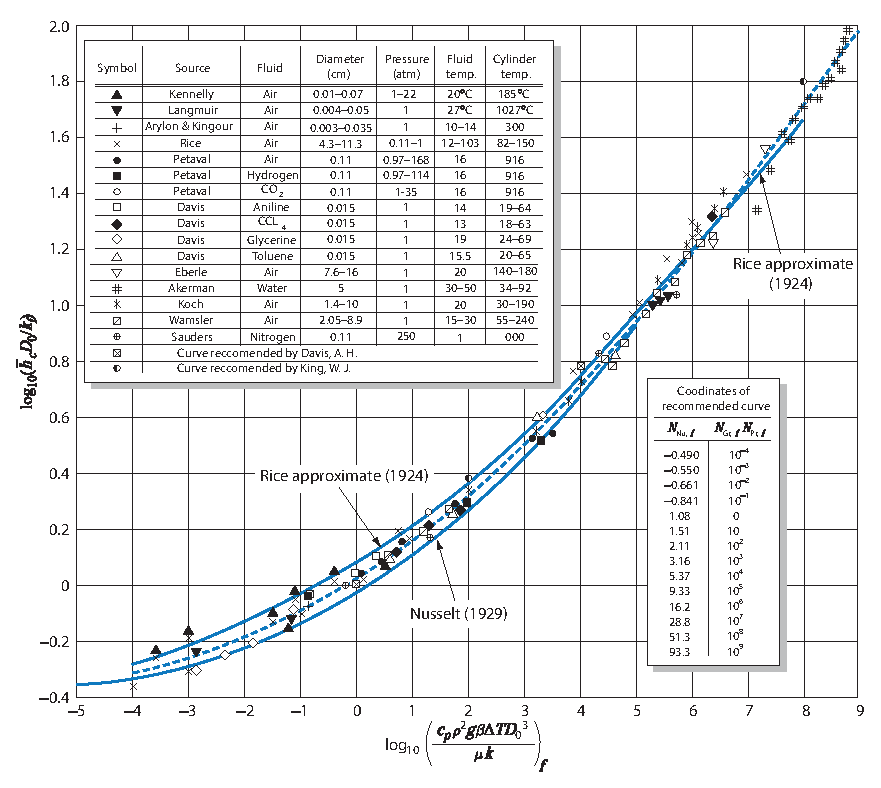
\includegraphics[width=\textwidth/2]{graf.eps}
    \caption{Correlación empírica para transferencia de calor en cilindros horizontales con gases y líquidos.\cite{kreith2011principles}}
    \label{graf:NusseltNaturalConvectionHorizontalCilinder}
\end{figure}
\begin{figure}[htb!]
    \centering
    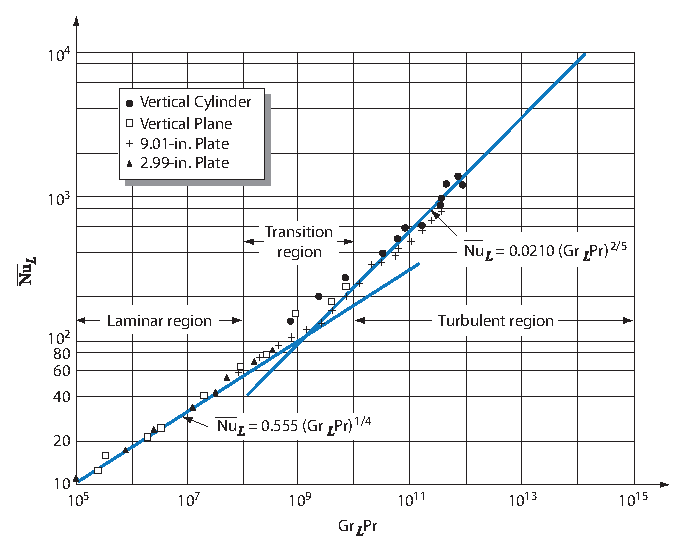
\includegraphics[width=\textwidth/2]{plaque.eps}
    \caption{Correlación empírica para transferencia de calor en cilindros y placas \emph{verticales}. \cite{kreith2011principles}}
    \label{graf:NusseltNaturalConvectionVerticalCilinderPlate}
\end{figure}
\subsubsection{Placas verticales}
Esta sección va exponer relaciones que coinciden con la realidad. Como en el Kreith, la dimensión característica aparece como subíndice para los parámetros adimensionales ($\Nusselt$, $\Reynolds$ etc.)

Placa o cilindro isotérmico vertical a una distancia $x$ de su comienzo con su capa limite
\begin{align*}\numberthis \label{eq:VerticalPlateOrCilinderPoint}
    h_{cx}&=0,508\Prandtl^{\frac{1}{2}}\sqrt[4]{\frac{\Grashof_x}{0,952+\Prandtl}}\frac{k}{x}\\
    \delta(x)&=4,3x\sqrt[4]{\frac{\Prandtl+0,56}{\Prandtl^2 \Grashof_x}}
\end{align*}
Integrando sobre la longitud característica $L$ y dividiendo por $L$ se puede obtener $\hcb=0,68\Prandtl^{\frac{1}{2}}\sqrt[4]{\frac{\Grashof_L}{0,952+\Prandtl}}\frac{k}{L}$.

Para una superficie plana sumergida en un metal fundido ($\Prandtl<0,03$) el promedio del número de $\Nusselt$ es
\begin{equation}
    \overline{\Nusselt}_L= \frac{\hcb L}{k}=0,68\sqrt[3]{\Grashof_L \Prandtl^2}
\end{equation}

en cambio, para régimen turbulento ($\Grashof>\num{e9}$) se recomienda:
\begin{equation}
    \overline{\Nusselt}_L=\frac{\hcb L}{k}=0,13\sqrt[3]{\Grashof \Prandtl}
\end{equation}

Para una placa inclinada a $\theta$ en el rango $\num{e5}<\Grashof_L\Prandtl\cos\theta<\num{e11}$ y $0\leq\theta\leq 89\grados $.
\begin{equation}
    \overline{\Nusselt_L}=0,56(\Grashof_L \Prandtl \cos\theta)
\end{equation}
\subsubsection{Placas horizontales}
Se tienen dos casos, cuando la gravedad ayuda a la transferencia de calor (\ref{eq:HorizontalPlateGravityHelping}) y cuando le juega en contra (\ref{eq:HorizontalPlateGravityBeingABitch}) donde $\ell$ toma el valor representativo $\frac{\textrm{Area de superficie}}{\textrm{Perímetro}}$:

\begin{align*}\numberthis\label{eq:HorizontalPlateGravityHelping}
    \overline{\Nusselt}_\ell &=0,54\sqrt[4]{\Rayleigh_\ell} \qquad (\num{e5}\lessapprox\Rayleigh_\ell \lessapprox\num{e7})\\
    \overline{\Nusselt}_\ell&=0,15\sqrt[3]{\Rayleigh_\ell} \qquad (\num{e7}\lessapprox\Rayleigh_\ell\lessapprox \num{e10})\\
\end{align*}
\begin{equation}\label{eq:HorizontalPlateGravityBeingABitch}
    \overline{\Nusselt}_\ell=0,27\sqrt[4]{\Rayleigh_\ell} \qquad (\num{e5}\lessapprox\Rayleigh_\ell \lessapprox \num{10e10})
\end{equation}




\subsection{Correlación empírica para cuerpos no-fuselados o \emph{bluff} con Convección forzada}
\textbf{Cuerpo no-fuselado}:\emph{Un cuerpo que tiene el frente ancho, aplanado, como en el caso de algunos vehículos de reentrada atmosférica.} 

\subsubsection{Cilindros}
$$C_D=\frac{F_D}{A_f\left( \rho U^2_\infty /2g_c\right)}$$
donde $D$ es el diámetro exterior, $L$ es la longitud del cilindro, $A_f$ es el área frontal proyectado,$U_\infty$ es la velocidad de la corriente libre.

Para un cilindro se puede calcular $h_c$ sobre un punto cualquiera a $\theta$ grados de la horizontal que \emph{enfrenta} el flujo \textbf{laminar adherido}. 
\begin{equation} \label{eq:nusselt}
    \Nusselt_D(\theta)=\frac{h_c(\theta) D}{k}=1,14\sqrt{\frac{\rho U_\infty D}{\mu}}\cdot \Prandtl^{0.4} \left[ 1- \left(\frac{\theta}{90}\right)^3 \right] 
\end{equation}
El coeficiente de transferencia de calor es máximo en el punto estancamiento que enfrenta al flujo. A números de Reynolds mas altos se generan eddies en la parte posterior del cilindro que no mezclan efectivamente con el flujo principal disminuyendo así la transferencia de calor en $\theta=180$.

El problema se vuelve complejo para Reynolds altos. 
\begin{equation} \label{eq:nusseltmean}
    \overline{\Nusselt}_D=\frac{\hcb D}{k}=C\left(\frac{U_\infty D}{\nu}\right)^m \Prandtl^n \left( \frac{\Prandtl}{\Prandtl_s}\right)^{0.25}
\end{equation}
evaluado con $n=0,37$ para $\Prandtl<10$ y $n=0,36$ para $\Prandtl>10$ 

\begin{table}[h]
\centering
\begin{tabular}{ccc}
\hline
$\Reynolds$                & C     & m   \\\hline
$1$ -- $40$              & $0,75$  & $0,4$ \\
$40$ -- $\num{1e3}$           & $0,51$  & $0,5 $\\
$\num{1e3}$ -- $\num{2e5}$      & $0,26$  & $0,6$ \\
$\num{2e5}$ -- $\num{1e6}$ & $0,076$ & $0,7$\\\hline
\end{tabular}
\label{tab:coeficientes1}
\caption{Coeficientes para la ecuación \ref{eq:nusseltmean}}
\end{table}

Si se tiene un cilindro que no esta en \emph{cross-flow} (caso $\vartheta=90\grados$ siendo $\vartheta$ el ángulo de \emph{guiñada} o \emph{yaw angle}):
\begin{equation}
    \overline{\Nusselt}_D=0,206\Reynolds^{0,63}_N \Prandtl^{0.36} \qquad 2500<\Reynolds_N<\Reynolds_\crit
\end{equation}
donde $\Reynolds_N=\Reynolds_D \sin \vartheta $ y $\Reynolds_\crit$ varía dependiendo de $\vartheta$ entre \num{2e4} para $\vartheta=15\grados$ y \num{2.5e5} para $\vartheta=45\grados$

En el rango $\num{2e5}<\Reynolds_D<\num{e6}$ el número de Nusselt es independiente de $\vartheta$
\begin{equation}
    \overline{\Nusselt}_D=0,012\Reynolds_D^{0,85}\Prandtl^{0,36}
\end{equation}

Un cuerpo prismático de sección no-circular en un medio gaseoso se puede describir con siguiente ecuación tomando $B$ y $n$ de tabla
\begin{equation}
    \overline{\Nusselt}_D=B\Reynolds_D^n
\end{equation}

Usar $\Nusselt_D=1,125\left( \Reynolds_D \Prandtl\right)^{0,413}$ para cilindros con flujo metal-liquido $\vartheta=90\grados$. Valido en el rango $1\leq\Prandtl\cdot \Reynolds_D\leq 100$. 

El \emph{aspect ratio} $\frac{L}{D}$ juega un rol para valores menores a $4$. Dentro de este rango y para valores de Reynolds $\num{7e4} < \Reynolds_D < \num{2.2e5}$
\begin{equation}
    \overline{\Nusselt}_D=0,123 \Reynolds_D^{0,651}+0,00416\left( \frac{L}{D} \right)^{-0,85} \Reynolds_D^{0,792}
\end{equation}b

\subsubsection{Esferas}
En el rango $25 < \Reynolds_D < \num{1e5}$ vale la siguiente ecuación para una esfera calentada o enfriada por un gas:
\begin{equation} \label{eq:nusseltspheregas}
    \overline{\Nusselt}_D=\frac{\bar{h}_cD}{k}=0,37\left( \frac{\rho D U_\infty}{\mu}\right)^{0,6}=0,37\Reynolds_D^{0,6} 
\end{equation}

Para un flujo de un \textbf{gas} $1,0<\Reynolds_D<25$:
\begin{equation}
    \hcb = c_pU_\infty \rho \left(\frac{2,2}{\Reynolds_D}+\frac{0,48}{\sqrt{\Reynolds_D}} \right)
\end{equation}

Si se quisiera modelar la transferencia de calor en un liquido (o un gas) para $3.5<\Reynolds_D<\num{7.6e4}$ y $0,7<\Prandtl<380$:

\begin{equation}
    \overline{\Nusselt}_D\!=\frac{\hcb D}{k}=2+\!\left(0,4 \sqrt{\Reynolds_D}+\!0,06\sqrt[3]{\Reynolds_D^2}\right) \Prandtl^{0,4}\sqrt[4]{\frac{\mu}{\mu_s}}
\end{equation}
donde $\mu_s$ es la viscosidad del fluido a la temperatura de la superficie de la esfera.

Por debajo del $\Reynolds_\crit$,  $100<\Reynolds_D<\num{2e5}$ la ecuación anterior es modificada:
\begin{equation}\label{eq:nusseltspheresubcrit}
    \overline{\Nusselt}_D=2+\left( \frac{\Reynolds_D}{4}+\num{3e-4}\Reynolds_D^{1,6}\right)^\frac{1}{2}
\end{equation}

Después del limite critico (seguimos con gases) $\num{4e5}<\Reynolds_D<\num{5e6}$ con $a=\num{5e-3}$, $b=\num{2,5e-10}$ y $c=\num{-3,1e-17}$
\begin{equation}
    \overline{\Nusselt}_D=430+a\Reynolds_D+b\Reynolds_D^2+c\Reynolds_D^3
\end{equation}

Ahora en el caso que se esté transfiriendo calor de una esfera a un metal liquido en el rango $\num{3.6e4}<\Reynolds_D<\num{2e5}$ tenemos:
\begin{equation}
    \overline{\Nusselt}_D=\frac{\hcb D}{k}=2+0,386 \left( \Reynolds_D \Prandtl\right)^{\frac{1}{2}}
\end{equation}

\subsubsection{Otros objetos no-fuselados}
Números de Nusselt para una placa plana de ancho $D$ normal al flujo incidente (\ref{eq:nusseltplacaplana}) y un cilindro de sección semi-circular (lado curvo enfrentando el flujo) (\ref{eq:nusseltsemicilindro}) para $1,0<\Reynolds_D<\num{4e5}$:
\begin{equation}\label{eq:nusseltplacaplana}
    \overline{\Nusselt}_D=\frac{\hcb D}{k}=0,20\Reynolds^{\frac{2}{3}}_D
\end{equation}
\begin{equation}\label{eq:nusseltsemicilindro}
    \overline{\Nusselt}_D=\frac{\hcb D}{k}=0,16\Reynolds^{\frac{2}{3}}_D
\end{equation}

Para un disco orientado con su eje en la dirección de un flujo, valido en $5000<\Reynolds_D<\num{5e4}$:
\begin{equation}
    \overline{\Nusselt}_D=1,05\Reynolds_D^{\frac{1}{2}} \Prandtl^{0,36}
\end{equation}

Los datos experimentales obtenidos para una placa cuadrada orientada con guiñada $\vartheta\in [0\grados,45\grados]$ y ángulo de ataque $\vartheta_{\textrm{pitch}}\in[25\grados,90\grados]$ increíblemente tiene correlación con una sola ecuación (error=$\pm 5\%$):
\begin{equation}
    \frac{\hcb \Prandtl^{\frac{2}{3}}}{c_p\rho U_\infty}=\frac{0,930}{\sqrt{\Reynolds_L}}
\end{equation}

 \section{Convección Interna Laminar}
\subsection{Correlaciones empíricas}

Se comienza definiendo el diámetro hidráulico para poder aplicar las correlaciones a secciones que no son cuadradas ni circulares
\begin{equation}
    D_H=4\cdot \frac{\textrm{Sección de flujo}}{\textrm{Perimetro mojado}}
\end{equation}

Luego se define un valor que se usa seguido como criterio para las correlaciones $\Lambda$:
\[
\Lambda = \frac{\Reynolds_{D_H}\Prandtl D_H}{L}
\]

{\bf Ductos \emph{cortos} circulares o rectangulares.}

Si se trata el ducto rectangular corto con la hipótesis de placas planas
\begin{equation}
    \overline{\Nusselt}_{D_H}=-\frac{\Lambda}{4}\ln \left( 1 - 2,654 \Prandtl^{0,167} \Lambda^{-,5}\right)
\end{equation}
 \section{Intercambiadores de Calor}
El subíndice $c$ se refiere a \emph{cold}, $h$ a \emph{hot}. 
\begin{equation}
    q=(\dot{m}c_p)(T_{c,\salida}-T_{c,\entrada})
\end{equation}

\emph{Overall heat transfer coeficcient:}
\begin{equation}
    q=UA(T_h-T_c)
\end{equation}
\subsection{Diferencia de temperatura \textit{Log-mean}}
La temperatura varía según la dirección del flujo. Para obtener el coeficiente de transferencia de calor se tiene que integrar la siguiente expresión a lo largo del tubo(s).

\[ \di q=U\di A\Delta T
\]
Si $U$ es constante y no hay cambios en energía cinética, entonces 
\begin{equation}
    \di q = - \dot{m}_h c_{p,h} \di T_h = \pm \dot{m}_c c_{p.c} \di T_c = U \di A (T_h-T_c)
\end{equation}
donde el signo $\pm$ depende si los flujos son paralelos ($+$) o en \emph{counterflow} ($-$).


\begin{equation}
    q=UA\frac{\Delta T_a-\Delta T_b}{\ln (\Delta T_a\Delta T_b)}
\end{equation}
donde $\Delta T=T_h - T_c$.

\subsubsection*{Promedio logarítmico para intercambiadores tipo \textit{shell}}
El subíndice $s$ se refiere a una propiedad del \textit{shell}.

Promedio generalizado con factor de corrección
\begin{equation}
    \Delta T_{\promedio}=F\cdot\frac{\Delta T_a-\Delta T_b}{\ln (\Delta T_a\Delta T_b)}
\end{equation}

\subsection{Efectividad de Intercambiador}
La ecuación generalizada para intercambiadores de calor:


\begin{equation}
    q=UA\Delta T_{\promedio}
\end{equation}

Ahora presentamos la \emph{efectividad} $\efic$ que es la razón de calor intercambiado al calor intercambiado máximo posible (largo infinito).


\begin{align}
    \efic &= \frac{C_h (T_{h,\entrada}-T_{h,\salida})}{C_{\min}(T_{h,\entrada}-T_{c,\entrada})} \\
\efic &= \frac{C_c (T_{c,\salida}-T_{c,\entrada})}{C_{\min}(T_{h,\entrada}-T_{c,\entrada})} 
\end{align}
donde $C_{\min}$ es la menor de las magnitudes $\dot{m}_h c_{ph}$ y $\dot{m}_c c_{pc}$.

\begin{equation}
    q= \efic C_{\min}(T_{h,\entrada}-T_{c,\entrada})
\end{equation}

\begin{equation}
    \efic = \frac{1-\exp\left(\frac{-UA(1+C_{\min}/C_{\max})}{C_{\min}}\right)}{1+C_{\min}/C_{\max}}
\end{equation}


\subsection{\textit{Fouling}}

Factor \emph{fouling}
\begin{equation}
    R_d=\frac{1}{U_d}+\frac{1}{U}
\end{equation}
donde $U_d$ es el coeficiente de transmisión de calor después de ocurrir el \emph{fouling}.
 \section{Radiación}

\subsection{Cuerpos negros}

\begin{equation}
    E_{b}(T,\lambda)=\frac{C_1}{\lambda^5 (e^{C_1/\lambda T} -1)}
\end{equation}

\begin{equation}
    \frac{\di E_{b}(T,\lambda)}{\di \lambda}=0 \quad \Rightarrow \quad \lambda_{max} T = b= \num{2,898e-3} \si{\milli \kelvin}
\end{equation}

La emisión total de radiación por unidad de superficie es:
\begin{equation}
    E_b(T) = \frac{q_r}{A} = \sigma T^4
\end{equation}
donde $\sigma=\SI{5,670e-8}{\watt \per \meter \squared \kelvin^4 } $ es el constante de Stefan-Boltzmann.

Para determinar cual longitud de onda a la que el poder emisivo monocromático es máximo
\begin{equation}
    \frac{E_b (T,\lambda)}{E_b (T,\lambda_{max})}=\left( \frac{\num{2,898e-3}}{\lambda T}\right)^5 \left( \frac{\exp(4,965)-1}{\exp(\frac{0,014388}{\lambda T})-1} \right)
\end{equation}

\subsection{Intensidad de radiación}
Unidad de ángulo solido: Steradiano (sr)

\begin{equation}
    \di \omega = \frac{\di A_n}{r^2} = \sin \theta \di \theta \di \phi
\end{equation}

\subsection{Propiedades de la radiación}

Absorción + reflectividad + transimisión = 1
\[\alpha + \rho +\tau = 1 \]

Cuerpos opacos no transmiten radiación incidente $\Rightarrow \tau=0$. Cuando un cuerpo es un reflector perfecto entonces $\rho=1$.

\[ 
\varepsilon = \frac{E(T)}{E_b(T)} = \frac{E(T)}{\sigma T^4}
\]

{\bf Equilibrio entre tierra y sol} Encontrar $T_{tierra}$:

$T_{sol}=5778K, \quad R_{ts}=\SI{149,6e9}{\meter}, \quad R_T=6371 km,\quad R_S=695508km$, $albedo\approx0,35$, $\, \epsilon_{tierra} \approx 0,612$

Buscamos los steradianes de la tierra respecto el sol: $\omega=\frac{A_T}{R_{ts}^2}=\num{5,698e-9}$

Busco emitancia del sol y potencia radiada total:
$E=\sigma (5778^4) \Rightarrow P_{sol}=A_{sol}E=\SI{3,8e26}{\watt}$ Si divido por $4\pi$ obtengo intensidad radiante $I_e=[W/sr]$

y luego para calcular la intensidad de la radiación del sol sobre la tierra:
$I=\frac{P_{sol}}{A_{ts}}=\frac{P_{sol}}{4\pi R_{ts}^2}=1366\si{\watt \meter^{-2}}$

La energía absorbida por la tierra se puede calcular de dos formas:
$q_r=I\cdot \pi R_T^2=I_e\cdot \omega=\num{1,74e17}\si{\watt} $

Tomando en cuenta que la tierra es un cuerpo gris: 
$E_{absorbido}=q_r(1-albedo)$ y lo que emite: $E_{emite}=4\pi \epsilon R_T^2 \sigma T_{tierra}^4$.\footnote{La tierra absorbe luz en un plano e irradia como una esfera} Planteando $E_{emit}=E_{abs}$
\[ T_{tierra} = \sqrt[4]{\frac{q_r(1-albedo)}{4\pi \epsilon R_T^2 \sigma}}\approx 283\, K \approx 10^\circ \textrm{C}\]


 \newcommand{\air}{\textrm{aire}}
\onecolumn
\section{Appendix}
\subsection{Correlaciones empíricas para aire seco a nivel del mar}
Datos discretos obtenidos de Engineering Toolbox. Correlacion calculado usando \verb|nlinfit| en \Matlab. Error relativo es menor a 0,006\% para todas las formulas en el rango dado usando los coeficientes mostrados. Unidades estándares (SI).


\begin{align}
\beta_\air &\approx 0,0037-\num{1,43e-5}T+\num{6,58e-8}T^2 \qquad T\in [-80,40]\celsius \\
\rho_\air &\approx  \num{2,22e-5}T^2-0,0049T+1,29\qquad T\in [-80,40]\celsius \\
k_\air &\approx 0,0241 + \num{7.98e-5}T-\num{3,84e-8}T^2 \qquad T\in [-100,100]\celsius \\
\mu_\air &\approx \num{1,72}{-5} +\num{5e-8}T-\num{4,34e-11}T^2\qquad T\in [-100,100]\celsius \\
c_{p_\air} &\approx 1004 + 0,0385T-\num{2,63e-4}T^2 \qquad T\in [-100,100]\celsius \\
\Prandtl_\air &\approx 0,716 -\num{2,61e-4}T  \qquad T\in [-100,100]\celsius
\end{align}
 \bibliography{labibliografia} % Indica archivo


\end{document}










\onecolumn
\subsection*{Duda fluidos}
En algun punto de la materia\footnote{Filminas 1 v2 INTRO. Slide 19/44.} dijimos
\begin{equation} \label{eq:sigmaijMatrix}
\sigma_{ij}= -p\delta_{ij}+
\begin{bmatrix}
\sigma_{11}+p&\sigma_{21}&\sigma_{31} \\
\sigma_{12}&\sigma_{22}+p&\sigma_{32} \\
\sigma_{13}&\sigma_{23}&\sigma_{33}+p
\end{bmatrix} =-p\delta_{ij}+S_{ij}
\end{equation}
donde $p$ es la presion mecanica.

En el apunte de las ecuaciones locales, entre la ecuación 5.9 y 5.10 llegamos a
\begin{equation}
S_{kk} =\left(\lambda +\frac{2}{3}\mu \right)e_{kk}
\end{equation}

Y finalmente se afirma que la traza de $S_{ij}$ es nula porque ``esta contenida en $p$". Esto es lo mismo que decir que $\sigma_{11}=\sigma_{22}=\sigma_{33}=-p$. 

Mi pregunta es si ``los componentes de la traza de $\sigma_{ij}$ son siempre idénticos?"

%% RESPUESTA%%%%%%%%%%%%%%%%%%%%%%%%%%%%%%
\subsection*{Respuesta}
\textbf{La respuesta es no.}
Si bien tenes a $-p$ en todas las direcciones principales,  lo cual daria que los $\sigma_{(k)(k)}$ son iguales en algunos flujos puede haber gradientes de la velocidad en la direccion de la misma, esos esfuerzos aparecen en las componentes principales de $\sigma$.
%%%%%%%%%%%%%%%%%%%%%%%%%%
%%%%%%%%%%%%%%%%%%%%%%%%%%
\subsection*{Continuación}
Siguiendo ese hilo... Es verdad que
\begin{equation}
p=\pe - S_{kk} = \pe - \left(\lambda +\frac{2}{3} \right)e_{kk}
\end{equation}
Para fluidos simples, newtonianos vale:
\begin{equation}
    S_{ij} = \lambda e_{kk} \delta_{ij} + 2\mu e_{ij}
\end{equation}

Entonces según \ref{eq:sigmaijMatrix} tenemos:
\[
  \sigma_{ij}= -\left[\pe -\left(\lambda+ \frac{2}{3}\mu \right)e_{kk}\right]\delta_{ij}+\lambda e_{kk} \delta_{ij} + 2\mu e_{ij} = -\pe \delta_{ij} + 2\lambda e_{kk}\delta_{ij}+2\mu e_{ij}+\frac{2}{3}\mu e_{kk}\delta_{ij}
\]
Dado que los componentes de la traza de $S_{ij}$ no son idénticos no se puede suponer que la traza de $S_{ij}$ es nula.

Nos queda entonces que para flujos compresibles no nos queda otra opcion mas que expresar la ecuación de Navier--Stokes con la viscosidad de volumen $\lambda$.